\documentclass[12pt]{article}\usepackage[]{graphicx}\usepackage[]{color}
%% maxwidth is the original width if it is less than linewidth
%% otherwise use linewidth (to make sure the graphics do not exceed the margin)
\makeatletter
\def\maxwidth{ %
  \ifdim\Gin@nat@width>\linewidth
    \linewidth
  \else
    \Gin@nat@width
  \fi
}
\makeatother

\definecolor{fgcolor}{rgb}{0.345, 0.345, 0.345}
\newcommand{\hlnum}[1]{\textcolor[rgb]{0.686,0.059,0.569}{#1}}%
\newcommand{\hlstr}[1]{\textcolor[rgb]{0.192,0.494,0.8}{#1}}%
\newcommand{\hlcom}[1]{\textcolor[rgb]{0.678,0.584,0.686}{\textit{#1}}}%
\newcommand{\hlopt}[1]{\textcolor[rgb]{0,0,0}{#1}}%
\newcommand{\hlstd}[1]{\textcolor[rgb]{0.345,0.345,0.345}{#1}}%
\newcommand{\hlkwa}[1]{\textcolor[rgb]{0.161,0.373,0.58}{\textbf{#1}}}%
\newcommand{\hlkwb}[1]{\textcolor[rgb]{0.69,0.353,0.396}{#1}}%
\newcommand{\hlkwc}[1]{\textcolor[rgb]{0.333,0.667,0.333}{#1}}%
\newcommand{\hlkwd}[1]{\textcolor[rgb]{0.737,0.353,0.396}{\textbf{#1}}}%

\usepackage{framed}
\makeatletter
\newenvironment{kframe}{%
 \def\at@end@of@kframe{}%
 \ifinner\ifhmode%
  \def\at@end@of@kframe{\end{minipage}}%
  \begin{minipage}{\columnwidth}%
 \fi\fi%
 \def\FrameCommand##1{\hskip\@totalleftmargin \hskip-\fboxsep
 \colorbox{shadecolor}{##1}\hskip-\fboxsep
     % There is no \\@totalrightmargin, so:
     \hskip-\linewidth \hskip-\@totalleftmargin \hskip\columnwidth}%
 \MakeFramed {\advance\hsize-\width
   \@totalleftmargin\z@ \linewidth\hsize
   \@setminipage}}%
 {\par\unskip\endMakeFramed%
 \at@end@of@kframe}
\makeatother

\definecolor{shadecolor}{rgb}{.97, .97, .97}
\definecolor{messagecolor}{rgb}{0, 0, 0}
\definecolor{warningcolor}{rgb}{1, 0, 1}
\definecolor{errorcolor}{rgb}{1, 0, 0}
\newenvironment{knitrout}{}{} % an empty environment to be redefined in TeX

\usepackage{alltt}
\usepackage{amsmath}
\usepackage{amsthm}
\usepackage{graphicx,psfrag,epsf}
\usepackage{enumerate}
\usepackage{booktabs}
%\usepackage{natbib}
\RequirePackage[natbibapa]{apacite}
\usepackage{caption}
\usepackage{multirow}

%\pdfminorversion=4
% NOTE: To produce blinded version, replace "0" with "1" below.
\newcommand{\blind}{0}

% DON'T change margins - should be 1 inch all around.
\addtolength{\oddsidemargin}{-.7in}%
\addtolength{\evensidemargin}{-.5in}%
\addtolength{\textwidth}{1in}%
\addtolength{\textheight}{1.3in}%
\addtolength{\topmargin}{-.8in}%

\usepackage{float}    % for fig.pos='H'
\usepackage{rotfloat} % for sidewaysfigure

\usepackage[textwidth=1in, textsize=tiny]{todonotes}
%\usepackage[disable]{todonotes}

\newtheorem{thm}{Theorem}
\newtheorem{lem}{Lemma}

\newcommand{\Prob}{\text{Pr}}
\newcommand{\E}{\text{E}}
\newcommand{\Cov}{\text{Cov}}
\newcommand{\corr}{\text{corr}}
\newcommand{\Var}{\text{Var}}
\newcommand{\iid}{\stackrel{\text{iid}}{\sim}}
\newcommand{\tr}{\text{tr}}
\newcommand{\bm}{\mathbf}
\newcommand{\bs}{\boldsymbol}
\IfFileExists{upquote.sty}{\usepackage{upquote}}{}
\begin{document}

\def\spacingset#1{\renewcommand{\baselinestretch}%
{#1}\small\normalsize} \spacingset{1}


%%%%%%%%%%%%%%%%%%%%%%%%%%%%%%%%%%%%%%%%%%%%%%%%%%%%%%%%%%%%%%%%%%%%%%%%%%%%%%

\if0\blind
{
  \title{\bf Small sample methods for cluster-robust variance estimation and hypothesis testing in fixed-effect models}
  \author{\\James E. Pustejovsky\thanks{
    The authors thank Dan Knopf for helpful discussions about the linear algebra behind the cluster-robust variance estimator. Coady Wing,...}\hspace{.2cm}\\
    Department of Educational Psychology \\ 
    University of Texas at Austin\\ \\
    and \\ \\
    Elizabeth Tipton \\
    Department of Human Development \\ 
    Teachers College, Columbia University}
  \maketitle
} \fi

\if1\blind
{
  \bigskip
  \bigskip
  \bigskip
  \begin{center}
    {\LARGE\bf Small sample methods for cluster-robust variance estimation and hypothesis testing in fixed-effect models}
\end{center}
  \medskip
} \fi

\bigskip
\begin{abstract}
In longitudinal panels and other regression models with unobserved effects, fixed effects estimation is often paired with cluster-robust variance estimation (CRVE) in order to account for heteroskedasticity and un-modeled dependence among the errors. CRVE is asymptotically consistent as the number of independent clusters increases, but can be biased downward for sample sizes often found in applied work, leading to hypothesis tests with overly liberal rejection rates. One solution is to use bias-reduced linearization (BRL), which corrects the CRVE so that it is unbiased under a working model, and t-tests with Satterthwaite degrees of freedom. We propose a generalization of BRL that can be applied in models with arbitrary sets of fixed effects, where the original BRL method is undefined, and describe how to apply the method when the regression is estimated after absorbing the fixed effects. We also propose a small-sample test for multiple-parameter hypotheses, which generalizes the Satterthwaite approximation for t-tests. In simulations covering a variety of study designs that occur in economic applications, we find that conventional cluster-robust Wald tests can severely under-reject while the proposed small-sample test maintains Type I error very close to nominal level. 
\end{abstract}

\noindent%
{\it Keywords:} Robust Standard Errors, Clustering, Fixed-Effects, Small Samples
\vfill

\newpage
\spacingset{1.45} % DON'T change the spacing!

\section{INTRODUCTION}
\label{sec:intro}

In a wide array of economic analyses, interest centers on the parameters of linear regression models, estimated by ordinary or weighted least squares (OLS/WLS) from a sample of units that are correlated. 
Such correlation among units can arise from sampling aggregate units (e.g., countries, districts, villages), each of which contains multiple observations; from repeated measurement of an outcome on a common set of units, as in panel data; or from model misspecification, as in analysis of regression discontinuity designs \citep[e.g.,][]{Lee2008regression}. 
A common approach to inference in these settings is to use a cluster-robust variance estimator \citep[CRVE;][]{Arellano1987computing, Liang1986longitudinal, white1984asymptotic}.
The advantage of CRVEs is that they produce consistent standard errors and test statistics without imposing strong parametric assumptions about the dependence structure of the errors in the model.
Instead, the method relies on the weaker assumption that units can be grouped into clusters that are mutually independent. 
CRVEs are an extension to another economic mainstay, heteroskedasticity-robust variance estimators \citep{eicker1967limit, Huber1967behavior, White1980heteroskedasticity}, which are used to account for non-constant variance in regression models with independent errors.
In the past decade, use of CRVE has become standard practice for applied micro-economic analysis, as evidenced by coverage in major textbooks and review articles \citep[e.g.,][]{Wooldridge2010econometric, Angrist2009mostly, Cameron2015practitioners}.

As a leading example of the application of CRVEs, consider a study of the effects on employment outcomes of several state-level policy shifts, where the policies were implemented at different time-points in each state. 
In a difference-in-differences analysis of state-by-year panel data, the policy effects would be parameterized in a regression model that includes indicator variables for each policy shift and perhaps additional demographic controls. It is also common to include fixed effects for states and time-periods in order to control for unobserved confounding in each dimension. 
The model could be estimated by OLS, with the fixed effects included as indicator variables; more commonly, the effects of the policy indicators would be estimated after absorbing the fixed effects, a computational technique that is also known as the fixed effects or within transformation \citep{Wooldridge2010econometric}. 
Standard errors would then be clustered by state to account for residual dependence in the errors from a given state, and these clustered standard errors would be used to test hypotheses regarding each policy or the set of policies.
The need to cluster the standard errors by state, even when including state fixed effects, was highlighted by \citet{Bertrand2004how}, who showed that to do otherwise can lead to inappropriately small standard errors and hypothesis tests with incorrect rejection rates. 

The consistency property of CRVEs is asymptotic in the number of independent clusters \citep{Wooldridge2003cluster}.
Recent methodological work has demonstrated that CRVEs can be biased downward and associated hypothesis tests can have Type-I error rates considerably in excess of nominal levels when based on samples with only a small or moderate number of clusters \citep[e.g.,][]{Webb2013wild}.
\citet{Cameron2015practitioners} provide a thorough review of this literature, including a discussion of current practice, possible solutions, and open problems. 
In particular, they demonstrate that small-sample corrections for t-tests implemented in common software packages such as Stata and SAS do not provide adequate control of Type-I error. 

\citet[see also \citealt{McCaffrey2001generalizations}]{Bell2002bias} proposed a method that improves the small-sample properties of CRVEs. 
Their method, called bias-reduced linearization (BRL), entails adjusting the CRVE so that it is exactly unbiased under a working model specified by the analyst, while also remaining asymptotically consistent under arbitrary true variance structures. 
Simulations reported by \citet{Bell2002bias} demonstrate that the BRL correction serves to reduce the bias of the CRVE even when the working model is misspecified. 
The same authors also proposed and studied small-sample corrections to single-parameter hypothesis tests using the BRL variance estimator, based on Satterthwaite \citep{Bell2002bias} or saddlepoint approximations \citep{McCaffrey2006improved}. 
\citet{Angrist2009effects} applied the BRL correction in an analysis of a longitudinal cluster-randomized trial with 35 clusters, observing that the bias correction makes a difference for inferences. 

Despite a growing body of simulation evidence that BRL performs well \citep[e.g.,][]{Imbens2015robust}, several problems with the method hinder its wider application. 
First, \citet{Angrist2009mostly} noted that the BRL correction breaks down (i.e., cannot be calculated) in some highly parameterized models, such as state-by-year panels that include fixed effects for states and for years.
Second, in models with fixed effects, the magnitude of the BRL adjustment depends on whether it is computed based on the full design matrix used in OLS estimation (i.e., including fixed effect dummies) or after absorbing the fixed effects. 
\citet{Cameron2015practitioners} noted that other methods of small-sample correction suffer from the same subtle problem of depending on arbitrary computational details.  
Third, extant methods for hypothesis testing based on BRL are limited to single-parameter constraints \citep{Bell2002bias, McCaffrey2006improved} and small-sample methods for multiple-parameter hypothesis tests remain lacking.
Multiple-parameter tests are used in a range of applications, including in panel data settings (e.g., Hausman tests for consistency of random effects estimators), seemingly unrelated regression models, and analysis of field experiments with multiple treatment groups.\todo{Could we cite empirical examples of each of these?}

This paper addresses each of these concerns in turn, with the aim of extending the BRL method so that is suitable for everyday econometric practice, including models with fixed effects. 
First, we describe an extension to the BRL adjustment that is well-defined in models with arbitrary sets of fixed effects, where existing BRL adjustments break down. 
Second, we demonstrate how to calculate the BRL adjustments so that they are invariant to whether the regression model is estimated including dummy fixed effects or after absorbing the fixed effects (i.e., using the within estimator) and identify conditions under which first-stage absorption of the fixed effects can be safely ignored. 
Finally, we propose a procedure for testing multiple-parameter hypotheses by approximating the sampling distribution of the Wald statistic by Hotelling's $T^2$ distribution with estimated degrees of freedom. The method is a generalization of the Satterthwaite correction proposed by \citet{Bell2002bias} for single parameter constraints.

Our work is related to a stream of recent literature that has examined methods for cluster-robust inference with a small number of clusters. 
\citet{Conley2011inference} proposed methods for hypothesis testing in a difference-in-differences setting where the number of treated units is small and fixed, while the number of untreated units increases asymptotically. 
\citet{Ibragimov2010tstatistic} proposed a method for constructing robust tests of scalar parameters that maintains the nominal Type-I error rate; however, their method requires that the target parameter be identified within each independent cluster and so it is not always applicable.  
\citet{Cameron2008bootstrap} investigated a range of bootstrapping procedures that provide improved Type-I error control in small samples, finding that a cluster wild-bootstrap technique was particularly accurate in small samples. 
Nearly all of this work has focused on single-parameter hypothesis tests only. 
For multiple-parameter constraints, \citet{Cameron2015practitioners} suggest an ad-hoc degrees of freedom adjustment and note, as an alternative, that bootstrapping techniques can in principle be applied to multiple-parameter tests. 
However, little methodological work has examined the accuracy of multiple-parameter tests.

The paper is organized as follows. The remainder of this section introduces our econometric framework and reviews the standard CRVE methods, as implemented in most software applications.
Section \ref{sec:BRL} reviews the original BRL correction and describes modifications that make it possible to implement BRL in a broad class of models with fixed effects.
Section \ref{sec:testing} discusses methods for hypothesis testing based on the BRL-adjusted CRVE. 
Section \ref{sec:simulation} reports a simulation study examining the null rejection rates of our proposed test for multiple-parameter constraints, where we find that the small-sample test offers drastic improvements over commonly implemented alternatives. 
Section \ref{sec:examples} illustrates the use of the proposed hypothesis tests in three examples that cover a variety of contexts in which CRVE is commonly used. 
Section \ref{sec:conclusion} concludes and discusses avenues for future work. 

\subsection{Econometric framework}

We consider a linear regression model of the form,
\begin{equation}
\label{eq:fixed_effects_ij}
\ {y}_{ij} = \bm{r}_{ij}' \bs\beta + \bm{s}_{ij}' \bs\gamma + \bm{t}_{ij}' \bs\mu + \epsilon_{ij} 
\end{equation}
where for observation $j$ in cluster $i$, $\bm{r}_{ij}$ is a vector of $r$ predictors of primary interest (e.g., policy variables) and any additional controls, $\bm{s}_{ij}$ is a vector of $s$ fixed effects that vary across clusters, and $\bm{t}_{ij}$ is a vector of $t$ fixed effects that are identified within clusters. In the state-policy example described in the introduction, the $\bm{r}_{ij}$ would include indicator variables for each policy change, as well as additional demographic controls; $\bm{s}_{ij}$ would include year fixed effects; and $\bm{t}_{ij}$ would indicate state fixed effects. Interest would center on testing hypotheses regarding the coefficients in $\bs\beta$ that correspond to the policy indicators, while $\bs\gamma$ and $\bs\mu$ would be treated as incidental. 

For developing theory, it is often easier to work with the matrix version of this model, in which
\begin{equation}
\label{eq:fixed_effects}
\bm{y}_i = \bm{R}_i \bs\beta + \bm{S}_i \bs\gamma + \bm{T}_i \bs\mu + \bs\epsilon_i,
\end{equation}
where for cluster $i$, $\bm{R}_i$ is an $n_i \times r$ matrix of focal predictors and controls; $\bm{S}_i$ is an $n_i \times s$ matrix describing fixed effects that vary across clusters, and $\bm{T}_i$ is an $n_i \times t$ matrix describing fixed effects that are identified only within clusters. The distinction between the covariates $\bm{R}_i$ versus the fixed effects $\bm{S}_i$ is arbitrary and depends on the analyst's inferential goals. However, the distinction between the two fixed effect matrices $\bm{S}_i$ and $\bm{T}_i$ is unambiguous, in that the within-cluster fixed effects satisfy $\bm{T}_h \bm{T}_i' = \bm{0}$ for $h \neq i$. 

We shall assume that $\E\left(\bs\epsilon_i\left|\bm{R}_i,\bm{S}_i, \bm{T}_i\right.\right) = \bm{0}$ and $\Var\left(\bs\epsilon_i\left|\bm{R}_i,\bm{S}_i,\bm{T}_i\right.\right) = \bs\Sigma_i$, for $i = 1,...,m$, where the form of $\bs\Sigma_1,...,\bs\Sigma_m$ may be unknown but the errors are independent across clusters. 
For notational convenience, let $\bm{U}_i = \left[\bm{R}_i \ \bm{S}_i \right]$ denote the set of predictors that vary across clusters, $\bm{X}_i = \left[\bm{R}_i \ \bm{S}_i \ \bm{T}_i \right]$ denote the full set of predictors, $\bs\alpha = \left(\bs\beta', \bs\gamma', \bs\mu' \right)'$, and $p = r + s + t$.
Denote the total number of individual observations by $N = \sum_{i=1}^m n_i$.
Let $\bm{y}$, $\bm{R}$, $\bm{S}$, $\bm{T}$, $\bm{U}$, $\bm{X}$, and $\bs\epsilon$ denote the matrices obtained by stacking their corresponding components, as in $\bm{R} = \left(\bm{R}_1' \ \bm{R}_2' \ \cdots \ \bm{R}_m'\right)'$. 

We assume that $\bs\beta$ is estimated by weighted least squares (WLS) using symmetric, full rank weighting matrices $\bm{W}_1,...,\bm{W}_m$. 
Clearly, the WLS estimator includes OLS as a special case (where $\bm{W}_i = \bm{I}_i$, an identity matrix), as well as feasible GLS.\footnote{
The WLS estimator also encompasses the estimator proposed by \citet{Ibragimov2010tstatistic} for clustered data. 
Assuming that $\bm{X}_i$ has rank $p$ for $i = 1,...,m$, their proposed approach involves estimating $\bs\beta$ separately within each cluster and taking the simple average of these estimates. 
The resulting average is equivalent to the WLS estimator with weights $\bm{W}_i = \bm{X}_i \left(\bm{X}_i'\bm{X}_i\right)^{-2} \bm{X}_i$.} 
In the latter case, it is assumed that $\Var\left(\bm{e}_i\left|\bm{X}_i\right.\right) = \bs\Phi_i$, where $\bs\Phi_i$ is a known function of a low-dimensional parameter. 
For example, an auto-regressive error structure might be posited to describe repeated measures on an individual over time. 
The weighting matrices are then taken to be $\bm{W}_i = \hat{\bs\Phi}_i^{-1}$, where the $\hat{\bs\Phi}_i$ are constructed from estimates of the variance parameter.
Finally, for analysis of data from complex survey designs, WLS may be used with sampling weights in order to account for unequal selection probabilities.

\subsection{Absorption}

The goal of most analyses is to estimate and test hypotheses regarding the parameters in $\bs\beta$, while the fixed effects $\bs\gamma$ and $\bs\mu$ are not of inferential interest. Moreover, estimating all of the parameters by WLS becomes computationally intensive and numerically inaccurate if the model includes a large number of fixed effects (i.e., $s + t$ large). 
A commonly implemented solution is to first absorb the fixed effects, which leaves only the $r$ parameters in $\bs\beta$ to be estimated. 
Section \ref{sec:BRL} examines the implications of absorption for application of the BRL adjustment. 
In order to do, we now formalize the absorption method.

To begin, denote the full block-diagonal weighting matrix as $\bm{W} = \text{diag}\left(\bm{W}_1,...,\bm{W}_m\right)$.
Let $\bm{K}$ be the $x \times r$ matrix that selects the covariates of interest, so that $\bm{X} \bm{K} = \bm{R}$ and $\bm{K}'\bs\alpha = \bs\beta$.
For a generic matrix $\bm{Z}$ of full column rank, let $\bm{M_Z} = \left(\bm{Z}'\bm{W}\bm{Z}\right)^{-1}$ and $\bm{H_Z} = \bm{Z}\bm{M_Z}\bm{Z}'\bm{W}$. 

The absorption technique involves obtaining the residuals from the regression of $\bm{y}$ on $\bm{T}$ and from the multivariate regressions of $\bm{U} = [\bm{R}\ \bm{S}]$ on $\bm{T}$. 
The $\bm{y}$ residuals and $\bm{R}$ residuals are then regressed on the $\bm{S}$ residuals. 
Finally, these twice-regressed $\bm{y}$ residuals are regressed on the twice-regressed $\bm{R}$ residuals to obtain the WLS estimates of $\bs\beta$. 
Let $\bm{\ddot{S}} = \left(\bm{I} - \bm{H_T}\right)\bm{S}$, $\bm{\ddot{R}} = \left(\bm{I} - \bm{H_{\ddot{S}}}\right)\left(\bm{I} - \bm{H_T}\right)\bm{R}$, and $\bm{\ddot{y}} = \left(\bm{I} - \bm{H_{\ddot{S}}}\right)\left(\bm{I} - \bm{H_T}\right)\bm{y}$. 
In what follows, subscripts on $\bm{\ddot{R}}$, $\bm{\ddot{S}}$,  $\bm{\ddot{U}}$, and $\bm{\ddot{y}}$ refer to the rows of these matrices corresponding to a specific cluster. 
The WLS estimator of $\bs\beta$ can then be written as
\begin{equation}
\label{eq:WLS}
\bs{\hat\beta} = \bm{M_{\ddot{R}}} \sum_{i=1}^m \bm{\ddot{R}}_i' \bm{W}_i \bm{\ddot{y}}_i. 
\end{equation}
This estimator is algebraically identical to the direct WLS estimator based on the full set of predictors, \[
\bs{\hat\beta} = \bm{K}'\bm{M_X} \sum_{i=1}^m \bm{X}_i' \bm{W}_i \bm{y}_i,
\]
but avoids the need to solve a system of $p$ linear equations.

In the remainder, we focus on the more general case in which fixed effects are absorbed before estimation of $\bs\beta$. For models that do not include within-cluster fixed effects, so that the full covariate matrix is $\bm{U} = \left[\bm{R} \ \bm{S}\right]$, all of the results hold after substituting $\bm{U}$ for $\bm{\ddot{R}}$. 

\subsection{Standard CRVE}

The WLS estimator $\bs{\hat\beta}$, has true variance
\begin{equation}
\label{eq:var_WLS}
\Var\left(\bs{\hat\beta}\right) = \bm{M_{\ddot{R}}}\left(\sum_{i=1}^m \bm{\ddot{R}}_i' \bm{W}_i \bs\Sigma_i \bm{W}_i\bm{\ddot{R}}_i\right) \bm{M_{\ddot{R}}},
\end{equation}
which depends upon the unknown variance matrices $\bs\Sigma_i$. 
A model-based approach to estimating this variance would involve assuming that $\bm\Sigma_i$ follows a structure defined by some low-dimensional parameter; for example, it may be assumed that the structure was hierarchical or auto-regressive. 
The model-based variance estimator would substitute estimates of $\bs\Sigma_i$ into (\ref{eq:var_WLS}).
However, if the model is misspecified, this estimator will be inconsistent and inferences based upon it will be invalid.

The CRVE involves estimating $\Var\left(\bs{\hat\beta}\right)$ empirically, without imposing structural assumptions on $\bs\Sigma_i$. 
While there are several versions of this approach, all can be written in the form
\begin{equation}
\label{eq:V_small}
\bm{V}^{CR} = \bm{M_{\ddot{R}}}\left(\sum_{i=1}^m \bm{\ddot{R}}_i'\bm{W}_i \bm{A}_i \bm{e}_i \bm{e}_i' \bm{A}_i' \bm{W}_i \bm{\ddot{R}}_i\right) \bm{M_{\ddot{R}}},
\end{equation}
where $\bm{e}_i = \bm{Y}_i - \bm{X}_i \bs{\hat\beta}$ is the vector of residuals from cluster $i$ and $\bm{A}_i$ is some $n_i$ by $n_i$ adjustment matrix. 

The form of these adjustment matrices parallels those of the heteroskedasticity-consistent (HC) variance estimators proposed by \citet*{MacKinnon1985some}. 
The most basic CRVE, described by \citet{Liang1986longitudinal}, uses $\bm{A}_i = \bm{I}_i$, an $n_i \times n_i$ identity matrix. 
Following \citet{Cameron2015practitioners}, we refer to this estimator as CR0. 
This estimator is biased towards zero because the cross-product of the residuals $\bm{e}_i \bm{e}_i'$ tends to under-estimate the true variance $\bs\Sigma_i$ in cluster $i$.
A rough bias adjustment is to take $\bm{A}_i = c\bm{I}_i$, where $c = \sqrt{(m/(m-1))}$; we denote this adjusted estimator as CR1. Some functions in Stata use a slightly different correction factor $c_S = \sqrt{(m N)/[(m - 1)(N - p)]}$; we will refer to the adjusted estimator using $c_S$ as CR1S. When $N >> p$, $c_S \approx \sqrt{m/(m-1)}$ and so CR1 and CR1S will be very similar.
The CR1 or CR1S estimator is now commonly used in empirical applications.

Use of these adjustments still tends to under-estimate the true variance of $\hat{\bs\beta}$ \citep{Cameron2015practitioners}. 
Analytic work and simulation studies indicate that the degree of bias depends not only on the number of clusters $m$, but also on features of the covariates in $\bm{X}$. Specifically, 
the bias tends to be larger when the covariates are skewed or unbalanced across clusters, or when clusters vary in size \citep{Carter2013asymptotic, MacKinnon2013thirty}. 
A more principled approach to bias correction would therefore take into account these features of the covariates. 
One such estimator uses adjustment matrices given by $\bm{A}_i = \left(\bm{I} - \bm{\ddot{R}}_i \bm{M_{\ddot{R}}}\bm{\ddot{R}}_i'\bm{W}_i\right)^{-1}$. This estimator, denoted CR3, closely approximates the jackknife re-sampling variance estimator \citep{Bell2002bias, Mancl2001covariance}.  
However, CR3 tends to over-correct the bias of CR0, while the CR1 estimator tends to under-correct. 
The next section describes in detail the BRL approach, which makes adjustments that are intermediate in magnitude between CR1 and CR3. 


\section{BIAS REDUCED LINEARIZATION}
\label{sec:BRL}

In contrast to the CR1 or CR3 estimators, the BRL correction for CRVE is premised on a ``working'' model for the structure of the errors, which must be specified by the analyst. 
Under a given working model, adjustment matrices $\bm{A}_i$ are defined so that the variance estimator is exactly unbiased.
We refer to this correction as CR2 because it is an extension of the HC2 variance estimator for regressions with uncorrelated errors, which is exactly unbiased when the errors are homoskedastic \citep{MacKinnon1985some}.
The idea of specifying a model may seem antithetical to the purpose of using CRVE, yet extensive simulation studies have demonstrated that the method performs better in small samples than any of the other adjustments, even when the working model is incorrect. (See Section \ref{sec:simulation} for a review of this literature.) 
Although the CR2 estimator may no longer be exactly unbiased when the working model is misspecified, its bias still tends to be greatly reduced compared to CR1 or CR0 (thus the name ``bias reduced linearization''). Furthermore, as the number of clusters increases, reliance on the working model diminishes. 
In a sense, CR2 provides necessary scaffolding in the small-sample case, which falls away when there is sufficient data.

Let $\bs\Phi_i$ denote a working model for the covariance of the errors in cluster $i$ (up to a scalar constant), with $\bs\Phi = \text{diag}\left(\bs\Phi_1,...,\bs\Phi_m\right)$. 
For example, following \citet{Bell2002bias} we might assume $\bs\Phi_i = \bm{I}_i$, i.e., that the errors are uncorrelated and homoskedastic. 
Alternatively, \citet{Imbens2015robust} suggested using a basic random effects (i.e., compound symmetric) structure, in which $\bs\Phi_i$ has unit diagonal entries and off-diagonal entries of $\rho$, with $\rho$ estimated using the OLS residuals \citep[see][p. 16]{Imbens2015robust}.

Based on a given working model, in the original formulation of \citet{Bell2002bias}, the BRL adjustment matrices are chosen to satisfy the criterion
\begin{equation}
\label{eq:CR2_criterion_BM}
\bm{A}_i \left(\bm{I} - \bm{H_X}\right)_i \bs\Phi \left(\bm{I} - \bm{H_X}\right)_i' \bm{A}_i'  =  \bs\Phi_i 
\end{equation}
where $\left(\bm{I} - \bm{H_X}\right)_i$ denotes the rows of $\bm{I} - \bm{H_X}$ corresponding to cluster $i$.
If the working model and weight matrices are both taken to be identity matrices, then the adjustment matrices simplify to $\bm{A}_i = \left(\bm{I}_i - \bm{X}_i\bm{M_X} \bm{X}_i'\right)^{-1/2}$, where $\bm{Z}^{-1/2}$ denotes the symmetric square-root of the matrix $\bm{Z}$. 
This formulation of $\bm{A}_i$ is problematic because, for some fixed effects models that are common in economic applications, Equation \ref{eq:CR2_criterion_BM} does not have a solution. 
In the next two subsections, we address two problems that arise in models with fixed effects, thereby articulating a BRL methodology that is suitable for a wide range of applications.

\subsection{Generalized Inverse}

The equality defining the $\bm{A}_i$ matrices cannot always be solved because it is possible that some of the matrices involved are not of full rank, and thus cannot be inverted. 
\citet{Angrist2009mostly} note that this problem arises in balanced state-by-year panel models that include fixed effects for states and for years. 
In order to address this concern, we provide an alternative criterion for the adjustment matrices that can always be satisfied. 
Instead of criterion (\ref{eq:CR2_criterion_BM}), we seek adjustment matrices $\bm{A}_i$ that satisfy:
\begin{equation}
\label{eq:CR2_criterion}
\bm{\ddot{R}}_i' \bm{W}_i \bm{A}_i \left(\bm{I} - \bm{H_X}\right)_i \bs\Phi \left(\bm{I} - \bm{H_X}\right)_i' \bm{A}_i' \bm{W}_i \bm{\ddot{R}}_i = \bm{\ddot{R}}_i' \bm{W}_i \bs\Phi_i \bm{W}_i \bm{\ddot{R}}_i.
\end{equation}
A variance estimator that uses such adjustment matrices will be exactly unbiased when the working model is correctly specified.

The above criterion (\ref{eq:CR2_criterion}) does not uniquely define $\bm{A}_i$. One solution, which produces symmetric adjustment matrices, uses
\begin{equation}
\label{eq:CR2_adjustment}
\bm{A}_i = \bm{D}_i' \bm{B}_i^{+1/2} \bm{D}_i,
\end{equation}
where $\bm{D}_i$ is the upper-right triangular Cholesky factorization of $\bs\Phi_i$, 
\begin{equation}
\label{eq:CR2_Bmatrix}
\bm{B}_i = \bm{D}_i\left(\bm{I} - \bm{H_X}\right)_i \bs\Phi \left(\bm{I} - \bm{H_X}\right)' \bm{D}_i',
\end{equation}
and $\bm{B}_i^{+1/2}$ is the symmetric square root of the Moore-Penrose inverse of $\bm{B}_i $. 
The Moore-Penrose inverse is well-defined and unique even when $\bm{B}_i$ is not of full rank \citep[][Thm. 9.18]{Banerjee2014linear}. These adjustment matrices satisfy criterion (\ref{eq:CR2_criterion}), as stated in the following theorem.

\begin{thm}
\label{thm:BRL_FE}
Let $\bm{L}_i = \left(\bm{\ddot{U}}'\bm{\ddot{U}} - \bm{\ddot{U}}_i'\bm{\ddot{U}}_i\right)$, where $\bm{\ddot{U}} = \left(\bm{I} - \bm{H_T}\right)\bm{U}$, and assume that $\bm{L}_1,...,\bm{L}_m$ have full rank $r + s$. Further assume that $\Var\left(\bs\epsilon_i\left|\bm{R}_i,\bm{S}_i,\bm{T}_i\right.\right) = \sigma^2 \bs\Phi_i$, for $i = 1,...,m$. Then the adjustment matrix $\bm{A}_i$ defined in (\ref{eq:CR2_adjustment}) and (\ref{eq:CR2_Bmatrix}) satisfies criterion (\ref{eq:CR2_criterion}) and the CR2 variance estimator is exactly unbiased.
\end{thm}

Proof is given in Appendix \ref{app:theorems}. If $\bm{B}_i$ is of full rank, then the adjustment matrices also satisfy the original criterion (\ref{eq:CR2_criterion_BM}). The main implication of Theorem \ref{thm:BRL_FE} is that the CR2 variance estimator remains well-defined, even in models with large sets of fixed effects.

\subsection{Absorption and Dummy Equivalence}

A problem with existing small-sample adjustments to CRVEs is that they can result in a different estimator depending upon if the fixed effects are estimated by OLS or are first absorbed. 
For example, this problem arises with the CR1S estimator because it uses a multiplicative correction to the residuals that depends on the total number of covariates estimated in the model. 
When fixed effects are included as indicators, the constant is calculated as $c_S = \sqrt{(mN) / [(m - 1)(N - p)]}$, where $p$ is the total number of covariates, including fixed effects. 
In contrast, if the fixed effects are absorbed, the constant is calculated as $c_S = \sqrt{(mN) / [(m - 1)(N - r)]}$, where $r$ is the number of covariates that are not absorbed. 
\citet{Cameron2015practitioners} highlight that this discrepancy can be substantial if the clusters are small. For instance, if each cluster includes $n_i = 2$ units, then the CR1S estimator based on estimating the fixed effects by OLS is over twice as large as the estimator based on the absorbed model.
Such differences between the correction based on OLS estimation of the fixed effects and the correction based on the absorbed model are problematic because the magnitude of the variance estimator should not depend on how the model estimates are calculated. 

Similar inconsistencies can arise when applying the BRL method in models with fixed effects. 
Consider the scenario in which absorption is used to estimate $\bs\beta$; here, the analyst might choose to calculate the CR2 correction based on the absorbed covariate matrix $\bm{\ddot{R}}$---that is, by substituting $\bm{H_{\ddot{R}}}$ for $\bm{H_X}$ in (\ref{eq:CR2_Bmatrix})---in order to avoid calculating the full projection matrix $\bm{H_X}$. 
However, this approach can lead to differences in the adjustment matrices compared to when the full model is estimated by OLS because it is based on a subtly different working model. 
Essentially, calculating CR2 based on the absorbed model amounts to assuming that the working model $\bs\Phi$ applies not to the model errors $\bs\epsilon$, but rather to the errors from the regression of $\bm{\ddot{y}}$ on $\bm{\ddot{R}}$.
We find this method of specifying the working model to be incoherent, and therefore recommend against taking it.
Rather, the CR2 adjustment matrices should be calculated based on a working model for the errors in the full regression model, following Equations (\ref{eq:CR2_adjustment}) and (\ref{eq:CR2_Bmatrix}) as stated. 

A drawback of using the CR2 adjustment matrices based on the full regression model is that it entails calculating the projection matrix $\bm{H_X}$ for the full set of $p$ covariates (i.e., including fixed effect indicators). Given that the entire advantage of using absorption to calculate $\hat{\bs\beta}$ is to avoid computations involving large, sparse matrices, it is of interest to find methods for more efficiently calculating the CR2 adjustment matrices. Some efficiency can be gained by using the fact that the residual projection matrix $\bm{I} - \bm{H_X}$ can be factored into components as $\left(\bm{I} - \bm{H_X}\right)_i = \left(\bm{I} - \bm{H_{\ddot{R}}}\right)_i \left(\bm{I} - \bm{H_{\ddot{S}}}\right) \left(\bm{I} - \bm{H_T}\right)$.

In certain cases, further computational efficiency can be achieved by computing the adjustment matrices after absorbing the within-cluster fixed effects $\bm{T}$ (but not the between-cluster fixed effects $\bm{S}$). 
Specifically, if the weights used for WLS estimation are the inverses of the working covariance model, so that $\bm{W}_i = \bs\Phi_i^{-1}$ for $i = 1,...,m$, then the adjustment matrices can be calculated without accounting for the within-cluster fixed effects. 
This result is formalized in the following theorem.  

\begin{thm}
\label{thm:absorb}
Let $\bm{\tilde{A}}_i = \bm{D}_i'\bm{\tilde{B}}_i^{+1/2} \bm{D}_i$, where 
\begin{equation}
\label{eq:CR2_B_tilde}
\bm{\tilde{B}}_i = \bm{D}_i\left(\bm{I} - \bm{H_{\ddot{R}}}\right)_i \left(\bm{I} - \bm{H_{\ddot{S}}}\right) \bs\Phi \left(\bm{I} - \bm{H_{\ddot{S}}}\right)' \left(\bm{I} - \bm{H_{\ddot{R}}}\right)_i' \bm{D}_i'.
\end{equation}
If $\bm{T}_i \bm{T}_k' = \bm{0}$ for $j \neq k$ and $\bm{W} = \bs\Phi^{-1}$, then $\bm{A}_i = \bm{\tilde{A}}_i$. 
\end{thm}

Proof is given in Appendix A.
The main implication of Theorem \ref{thm:absorb} is that the more computationally convenient formula $\bm{\tilde{B}}_i$ can be applied in the common case that the weighting matrices are the inverse of the working covariance model.

Following the working model suggested by \citet{Bell2002bias}, in which $\bs\Phi = \bm{I}$, the above theorem shows that the adjustment method is invariant to the choice of method for dealing with fixed effects so long as the model is estimated by OLS (i.e., $\bm{W} = \bm{I}$).
In this case, the CR2 adjustment matrices then simplify further to \[
\bm{A}_i = \left(\bm{I}_i - \bm{\ddot{U}}_i\left(\bm{\ddot{U}}'\bm{\ddot{U}}\right)^{-1}\bm{\ddot{U}}_i'\right)^{+1/2}. \]
In contrast, if the working model proposed by \citet{Imbens2015robust} is instead used, then the above theorem implies that the CR2 adjustments will differ if the model is estimated by OLS with dummies for fixed effects versus by using absorption.\todo{I'm not sure how important this point is, since the only scenario where the IK working model makes sense is for models WITHOUT cluster fixed effects.}

The two theorems of this section extend the BRL methodology described by \citet{Bell2002bias}, demonstrating how the CR2 adjustment can be computed efficiently---and from a coherent working model---for a broad range of commonly used regression models, including those with within- and between-cluster fixed effects.
The next section addresses a final set of concerns: how to conduct single- and multiple-parameter hypothesis tests using the CR2 estimator. 

\section{HYPOTHESIS TESTING}
\label{sec:testing}

The CR2 correction produces a CRVE that has reduced bias (compared to other CRVEs) when the number of clusters is small, leading to more accurate standard errors. However, standard errors are of limited inherent interest---rather, their main use is for the construction of hypothesis tests and confidence intervals.
Cluster-robust Wald-type test statistics are a function of the parameter estimates $\bs{\hat\beta}$ and the corresponding CRVE.
Conventional Wald tests are justified based on the asymptotic behavior of robust Wald statistics as the number of clusters grows large (i.e., as $m \to \infty$). 

Like the research on the bias of the CRVE estimator, evidence from a wide variety of contexts indicates that the asymptotic limiting distribution of these statistics may be a poor approximation when the number of clusters is small, even if corrections such as CR2 or CR3 are employed \citep{Bell2002bias, Bertrand2004how, Cameron2008bootstrap}. 
Like the bias of the CRVE estimator itself, the accuracy of the asymptotic approximations depends on design features such as the degree of imbalance across clusters, skewness or leverage of the covariates, and the similarity of cluster sizes \citep{McCaffrey2001generalizations, Tipton2015small-F, Webb2013wild, Carter2013asymptotic}. 
This provides motivation for development of general-purpose hypothesis testing procedures that have accurate rejection rates in small samples.

In this section, we develop a general method for conducting hypothesis tests based on CRVEs. We consider linear constraints on $\bs\beta$, where the null hypothesis has the form $H_0: \bm{C}\bs\beta = \bm{d}$ for fixed $q \times r$ matrix $\bm{C}$ and $q \times 1$ vector $\bm{d}$. 
The cluster-robust Wald statistic is then
\begin{equation}
\label{eq:Wald_stat}
Q = \left(\bm{C}\bs{\hat\beta} - \bm{d}\right)'\left(\bm{C} \bm{V}^{CR} \bm{C}'\right)^{-1}\left(\bm{C}\bs{\hat\beta} - \bm{d}\right),
\end{equation}
where $\bm{V}^{CR}$ is one of the cluster-robust estimators described in previous sections. 
The asymptotic Wald test rejects $H_0$ if $Q$ exceeds the $\alpha$ critical value from a chi-squared distribution with $q$ degrees of freedom. 
In large samples, it can be shown that this test has level $\alpha$. 
However, in practice it is rarely clear how large a sample is needed for the asymptotic approximation to be accurate. 

\subsection{Small-sample corrections for t-tests}
\label{subsec:t-tests}

Consider testing the hypothesis $H_0: \bm{c}'\bs\beta = 0$ for a fixed $r \times 1$ contrast vector $\bm{c}$. 
For this one-dimensional constraint, an equivalent to the Wald statistic given in (\ref{eq:Wald_stat}) is to use the test statistic $Z = \bm{c}'\bs{\hat\beta} / \sqrt{\bm{c}'\bm{V}^{CR}\bm{c}}$, which follows a standard normal distribution in large samples. 
In small samples, it is common to use the CR1 or CR1S estimator and to approximate the distribution of $Z$ by a $t(m - 1)$ distribution. 
\citet{Hansen2007asymptotic} provided one justification for the use of this reference distribution by identifying conditions under which $Z$ converges in distribution to $t(m-1)$ as the within-cluster sample sizes grow large, with $m$ fixed \citep[see also][]{Donald2007inference}. 
\citet{Ibragimov2010tstatistic} proposed a weighting technique derived so that that $t(m-1)$ critical values are conservative (leading to rejection rates less than or equal to $\alpha$).
However, both of these arguments require that $\bm{c}'\bs\beta$ be separately identified within each cluster. 
Outside of these circumstances, using $t(m-1)$ critical values can still lead to over-rejection \citep{Cameron2015practitioners}. 
Furthermore, using these critical values does not take into account that the distribution of $\bm{V}^{CR}$ is affected by the structure of the covariate matrix. 

An alternative t-test developed by \citet{Bell2002bias} involves using a $t(\nu)$ references distribution, with degrees of freedom $\nu$ estimated by a Satterthwaite approximation.
The Satterthwaite approximation \citep{Satterthwaite1946approximate} entails using degrees of freedom that are a function of the the first two moments of the sampling distribution of $\bm{c}' \bm{V}^{CR} \bm{c}$.
Theoretically, these degrees of freedom should be 
\begin{equation}
\label{eq:nu_Satterthwaite}
\nu = \frac{2\left[\E\left(\bm{c}'\bm{V}^{CR2}\bm{c}\right)\right]^2}{\Var\left(\bm{c}'\bm{V}^{CR2}\bm{c}\right)}.
\end{equation}
Expressions for the first two moments of $\bm{c}'\bm{V}^{CR2}\bm{c}$ can be derived under the assumption that the errors $\bs\epsilon_1,...,\bs\epsilon_m$ are normally distributed. 

In practice, both moments involve the variance structure $\bs\Sigma$, which is unknown. 
\citet{Bell2002bias} proposed to estimate the moments based on the same working model that is used to derive the adjustment matrices. 
This ``model-assisted'' estimate of the degrees of freedom is then calculated as 
\begin{equation}
\label{eq:nu_model}
\nu_{M} = \frac{\left(\sum_{i=1}^m \bm{p}_i' \bs\Phi \bm{p}_i\right)^2}{\sum_{i=1}^m \sum_{j=1}^m \left(\bm{p}_i' \bs\Phi \bm{p}_j\right)^2},
\end{equation}
where $\bm{p}_i = \left(\bm{I} - \bm{H_X}\right)_i'\bm{A}_i \bm{W}_i\bm{\ddot{R}}_i\bm{M_{\ddot{R}}} \bm{c}$.
\todo{Can we use $\bm{H_{\ddot{U}}}$ here instead?} 
Alternately, for any of the CRVEs one could instead use an ``empirical'' estimate of the degrees of freedom, constructed by substituting $\bm{e}_i \bm{e}_i'$ in place of $\bs\Sigma_i$. 
However, \citet{Bell2002bias} found using simulation that this plug-in degrees of freedom estimate led to very conservative rejection rates. 

The \citet{Bell2002bias} Satterthwaite approximation has been shown to perform well in a variety of conditions (see Section 4). 
These studies encompass a variety of data generation processes, covariate types, and weighting procedures. 
A key finding is that the degrees of freedom depend not only on the number of clusters $m$, but also on features of the covariates. 
When the covariate is balanced across clusters---as occurs in balanced panels with a dichotomous covariate with the same proportion of ones in each cluster---the degrees of freedom are $m - 1$ even in small samples. 
However, when the covariate is highly unbalanced---as occurs when the panel is not balanced or if the proportion of ones varies from cluster to cluster---the degrees of freedom can be considerably smaller. 
Similarly, covariates with large leverage points will tend to exhibit lower of degrees of freedom. 

By adjusting the degrees of freedom to account for these features, the Type I error rate of the test is nearly always less than or equal to the nominal $\alpha$, so long as the degrees of freedom are larger than 4 or 5 \citep{Bell2002bias, Tipton2015small-t}.
This is because when the degrees of freedom are smaller, the t-distribution approximation to the sampling distribution does not hold, and the Type I error can be higher than the stated $\alpha$ level.\footnote{When the degrees of freedom are smaller than 4 or 5, \citet{Tipton2015small-t} suggested using a smaller $\bs\alpha$ level for hypothesis testing in order to partially compensate. 
Although degrees of freedom this small may seem unlikely, they can easily arise in practice even when the number of clusters is moderate. For example, in a state-by-year panel with $m = 48$ states, the degrees of freedom can be quite small if a policy is only implemented in 10 percent of states.}
In comparison, the CR1 degrees of freedom (i.e., $m - 1$) are constant, and the test only performs well when in the cases in which the covariates are balanced.
Because the degrees of freedom are covariate-dependent, it is not possible to assess whether a small-sample correction is needed based solely on the total number of clusters in the data. 
Consequently, \citet{Tipton2015small-t} argued that t-tests based on CRVE should routinely use the CR2 variance estimator and the Satterthwaite degrees of freedom, even when $m$ appears to be large.


\subsection{Small-sample corrections for F-tests}
\label{subsec:F-tests}

Little research has considered small-sample corrections for multiple-constraint hypothesis tests based on cluster-robust Wald statistics.
Cameron and Miller highlight this problem, noting that some form of adjustment is clearly needed in light of the extensive work on single-parameter tests.
We now describe an approach to multi-parameter testing that closely parallels the Satterthwaite correction for t-tests.

Our approach is to approximate the sampling distribution of $Q$ by Hotelling's $T^2$ distribution (a multiple of an F distribution) with estimated degrees of freedom. To motivate the approximation, let $\bm{G} = \bm{C} \bm{M_{\ddot{R}}}\bm{\ddot{R}}'\bm{W}\bs\Phi\bm{W}\bm{\ddot{R}}\bm{M_{\ddot{R}}} \bm{C}'$ denote the variance of $\bm{C}\bs{\hat\beta}$ under the working model and observe that $Q$ can be written as \[
Q = \bm{z}' \bs\Omega^{-1} \bm{z},
\]
where $\bm{z} = \bm{G}^{-1/2}\left(\bm{C}\bs{\hat\beta} - \bm{d}\right)$ and $\bs\Omega = \bm{G}^{-1/2} \bm{C} \bm{V}^{CR2}\bm{C}'\bm{G}^{-1/2}$. 
Now suppose that $\eta \times \bs\Omega$ follows a Wishart distribution with $\eta$ degrees of freedom and a $q$-dimensional identity scale matrix. It then follows that
\begin{equation}
\label{eq:AHT}
\left(\frac{\eta - q + 1}{\eta q}\right) Q \ \dot\sim \ F(q, \eta - q + 1).
\end{equation}
We will refer to this as the approximate Hotelling's $T^2$ (AHT) test.
We consider how to estimate $\eta$ below.
This approximation is conceptually similar to the Satterthwaite approximation for one-dimensional constraints, and in fact reduces to the Satterthwaite approximation when $q = 1$. 
For $q > 1$, the test depends on the multivariate distribution of $\bm{V}^{CR2}$, including both variance and covariance terms. 

\citet{Tipton2015small-F} recently introduced this test for application in the special case of CRVE for meta-regression models.
Wishart approximations have been considered as approximations in several simpler models where special cases of CRVE are used.
\citet{Nel1986solution} proposed an AHT-type test for testing equality of multivariate means across two samples with unequal variance-covariance matrices \citep[i.e., the multivariate Behrens-Fisher problem; see also][]{Krishnamoorthy2004modified}.
\citet{Zhang2012twowayANOVA} followed a similar approach in developing a test for contrasts in analysis of variance models with unequal within-cell variance, which are particularly simple cases of linear models with heteroskedastic error terms. 
\citet{Zhang2012MANOVA} extended the method to multivariate analysis of variance models where the covariance of the errors differs across groups, a special case of model (\ref{eq:fixed_effects}) where the CR2 variance estimator has a particularly simple form. 
In each of these special cases, the robust variance estimator is a mixture of Wishart distributions that is well-approximated by a Wishart distribution with estimated degrees of freedom.
Additionally, \citet{Pan2002small} described an F-test for use in GEE models, which uses the Wishart approximation to the distribution of $\bm{V}^{CR0}$ but estimates the degrees of freedom using a different method than the one we describe below.

The contribution of the present paper is to extend the AHT test to the general setting of linear models with fixed effects and clustered errors. 
The remaining question is how to estimate the parameter $\eta$, which determines scalar multiplier and denominator degrees of freedom of the AHT test. 
To do so, we match the mean and variance of $\bs\Omega$ to that of the approximating Wishart distribution under the working variance model $\bs\Phi$, just as in the degrees of freedom for the t-test. 
The problem that arises in doing so is that it is not possible to exactly match both moments if $q > 1$.
Following \citet{Tipton2015small-F}, we instead match the mean and total variance of $\bs\Omega$---i.e., the sum of the variances of its entries.

Let $\bm{g}_1,...,\bm{g}_q$ denote the $q \times 1$ column vectors of $\bm{G}^{-1/2}$. 
Let \[
\bm{p}_{si} = \left(\bm{I} - \bm{H_X}\right)_i' \bm{A}_i \bm{W}_i \bm{\ddot{R}}_i \bm{M_{\ddot{R}}}\bm{C} \bm{g}_s \]
for $s = 1,...,q$ and $i = 1,...,m$.\todo{Possible to simplify $p_{si}$ by ignoring within-cluster fixed effects?} 
The degrees of freedom are then estimated under the working model as
\begin{equation}
\label{eq:eta_model}
\eta_M = \frac{q(q + 1)}{\sum_{s,t=1}^q \sum_{i,j=1}^m \bm{p}_{si}'\bs\Phi\bm{p}_{tj} \bm{p}_{ti}'\bs\Phi\bm{p}_{sj} + \bm{p}_{si}'\bs\Phi\bm{p}_{sj} \bm{p}_{ti}'\bs\Phi\bm{p}_{tj}}.
\end{equation}
If $q = 1$, then $\eta_M$ reduces to $\nu_M$ from Equation (\ref{eq:nu_model}).

This AHT F-test shares several features with the t-test developed by Bell and McCaffrey. As with the t-test, the degrees of freedom of this F-test depend not only on the number of clusters, but also on features of the covariates being tested. 
The degrees of freedom can be much lower than $m - 1$, particularly when the covariates being tested exhibit high leverage or are unbalanced across clusters. 
For example, if the goal is to test if there are differences across a three-arm, block-randomized experiment with clustering by block, the degrees of freedom will be largest (approaching $m - 1$) when the treatment is allocated equally across the three groups within each block. 
When the proportion varies across clusters, the degrees of freedom are reduced, potentially into ``small sample'' territory even when the number of clusters is large. 
% Outside of this simple example, it is generally more difficult to diagnose the cause of lower degrees of freedom in the multi-parameter case.\todo{Is this point necessary?}

Overall, throughout this section we have argued that AHT test performs well even with small numbers of clusters, that mispecification of the working model matters little, that differences between the AHT and standard test are driven by changes in the degrees of freedom, and that these degrees of freedom are impacted by covariate features.\todo{We haven't really made these points yet, have we?}
In the next section, we provide evidence for these claims through a careful review of prior simulation study results and through the results of a new simulation study based upon the conditions commonly found in economic applications.

\section{Simulation evidence}
\label{sec:simulation}

Evidence from several large simulation studies indicates that hypothesis tests based on the CR2 adjustment and estimated degrees of freedom substantially out-perform the procedures that are most commonly used in empirical applications.
However, existing simulations have focused almost entirely on single-parameter tests. 
In this section, we first review findings from previous simulations, with particular emphasis on the role of covariate features and sample size on the Type I error rates of these tests.
We then describe the design and results of a new simulation study, which focused on the rejection rates of multiple-parameter tests.
  Throughout, we refer to tests employing the CR2-corrected CRVE and estimated degrees of freedom as the ``AHT'' test; for t-tests, the estimated degrees of freedom are equivalent to the Satterthwaite approximation given in Equation (\ref{eq:nu_model}). 
We refer to tests employing the CR1 correction and $m - 1$ degrees of freedom as the ``standard'' test. 

\subsection{Review of previous simulation studies}

To date, four simulation studies have examined the performance of the CR2 t-test, across a total of nearly 100 parameter combinations and a range of application contexts.
\citet{Cameron2015practitioners} and \citet{Imbens2015robust} focused on conditions common in economics, while \citet{Bell2002bias} focused on those common in complex surveys and \citet{Tipton2015small-t} on those in meta-analysis. 
Table \ref{tab:simulation_summary} summarizes the results of these studies.
Some of the studies focused on policy dummies in the balanced case, while others varied the degree of balance; still others examined continuous covariates that are symmetrically distributed, as well as those with high skew and leverage.
These studies also examined the role of the number of clusters, with values ranging from 6 to 50, as well as the number of observations per clusters (from 1 to roughly 260).
Finally, the studies used a range of both true error structures (including various combinations of heteroskedasticity and clustering) and estimation strategies (including different 'working' models), including scenarios in which the working model differed from the true error structure.
Finally, while most previous studies focused on OLS estimation, one study \citep{Tipton2015small-t} examined the performance of t-tests based on WLS estimation.\todo{Beth, is there any way to condense the four columns under ``Variable type''? If you change it in the Excel file I will modify this table to match.}\todo{Beth, what is the difference between IK2015 Table 1 vs Table 2?}

\begin{sidewaystable}
\small
\caption{Type I error rates of t-tests based on CRVE}
\label{tab:simulation_summary}
\begin{tabular}{lc cccc c cccc} 
\toprule
 & & \multicolumn{4}{c}{Data generation}  & & \multicolumn{4}{c}{Type I error ($\alpha = .05$)} \\ \cmidrule{3-6} \cmidrule{8-11}
 & & & & \multirow{2}{1.5cm}{Error structure} & \multirow{2}{1.5cm}{Covariate type(s)} & \multirow{2}{1.5cm}{Working model} & \multicolumn{2}{c}{Standard} & \multicolumn{2}{c}{AHT} \\ 
Article & Table & $m$ & $n$ & & & & Min & Max & Min & Max \\ \midrule
BM 2002 & 2 & 20 & 10 & RE(3) & c[50\%, 15\%, M], o[M] & I & .05 & .16 & .03 & .05 \\
CM 2015 & 2 & 6-50 & ~260 & IPUMS-CPS & c[50\%] & RE & .07 & .11 & .05 & .05 \\ \midrule
\multirow{7}{1.5cm}{IK 2015} & 1 & 30 & 1 & H(5) & c[10\%] & I & .12 & .22 & .01 & .05 \\
& 2 & 30 & 1 & H(5); LN & c[10\%] & I & .07 & .32 & .00 & .13 \\
& 3 & 30 & 1 & H(5) & c[50\%] & I & .05 & .05 & .05 & .05 \\
& 4 & 5-10 & 10-60 & RE; RE+H & c[M] & I; RE & .08 & .13 & .03 & .06 \\
& 5 & 50 & 6 & RE & c[50\%] & I; RE & .06 & .06 & .05 & .05 \\ 
& 5 & 50 & 6 & RE; RE+H & c[6\%] & I; RE & .15 & .23 & .01 & .05 \\
& 5 & 50 & 6 & RE & c[K] & I; RE & .13 & .13 & .03 & .03 \\ \midrule
\multirow{8}{1.5cm}{T 2015} & 1 & 10-40 & 1-10 & RE + C(9) & c[50\%] & H & .05 & .05 & .04 & .05 \\
& 1 & 10-40 & 1-10 & RE + C(9) & c[15\%] & H & .10 & .15 & .04 & .05 \\
& 1 & 10-40 & 1-10 & RE + C(9) & o[10\%] & H & .04 & .19 & .04 & .06 \\
& 1 & 10-40 & 1-10 & RE + C(9) & c[M] & H & .07 & .13 & .04 & .05 \\
& 1 & 10-40 & 1-10 & RE + C(9) & o[M] & H & .06 & .12 & .04 & .06 \\ 
& 1 & 10-40 & 1-10 & RE + C(9) & o[K] & H & .03 & .28 & .01 & .04 \\
& 2 & 20 & 1-10 & RE + C(9) & c[10\%,M], o[10\%, M] & H & .01 & .12 & .01 & .06 \\
& 2 & 20 & 1-10 & RE + C(9) & c[30\%,M], o[30\%, M] & H & .02 & .06 & .01 & .06 \\
\bottomrule
\end{tabular}



\caption*{Table refers to the table within the relevant article. $m$ is the number of clusters; $n$ is the number of observations within each cluster; c indicates cluster-level covariate, while o indicates observation-level covariate; \% = percent taking value of one; H = heteroskedastic; RE = random effects (Moulton factor); C = correlated errors; (\#) indicates number of different models tested.}
\end{sidewaystable}

Table \ref{tab:simulation_summary} also indicates the range of Type I error rates observed across the conditions studied in each of the simulation studies, with values given for both the standard and AHT tests.
Across studies, the Type I error for the standard t-test ranges from .01 to .34 for a stated $\alpha$ level of .05.
These values are particularly far above nominal when the covariate tested is unbalanced, skewed (i.e., high leverage), or when the number of observations per cluster varies. 
Although not reported in the table, high Type I error rates occur not only when the number of clusters is very small, but also at moderate sizes when the covariate is unbalanced or skewed. 

In comparison, the AHT t-test performs considerably better across the range of conditions studied, with Type I error rates ranging between 0.01 and 0.13.
Notably, the largest value observed here is from \citet{Imbens2015robust}, who do not break results out by degrees of freedom. 
Given the condition studied (30 clusters, with only 3 having a policy dummy), it is quite possible that the degrees of freedom are below the cut-off of 4 or 5 at which others have shown the t-test approximation can fail \citep{Tipton2015small-t}. 
Putting this value aside, the maximum Type I error observed in these conditions is 0.06, only slightly higher than nominal.
Crucially, these nearly nominal Type I error rates hold even when the working model is far from the true error structure, and for various types of covariates.
This is because the AHT test takes into account covariate features in the degrees of freedom, which can be far less than $m - 1$.

In comparison to the t-test, the AHT F-test has only been studied in a single simulation focused on the meta-analytic case \citep{Tipton2015small-F}.
Although this study focused only on the use of CRVE with WLS estimation, it was comprehensive in other regards.
In particular, it examined the effects of the number of covariates in the model (up to $p = 5$) and the number of constraints tested ($q = 2,3,4,5$), including cases in which $p = q$ and in which $q < p$. 
The simulations also examined models with various combinations of covariate types, including both balanced and unbalanced indicator variables, as well as symmetric or skewed continuous covariates.
Like \citet{Tipton2015small-t}, these simulations focused on true correlation structures that included heteroskedasticity, clustering (i.e., a cluster specific random effect), and correlated errors.
The working models were then chosen to be far from the true error structure (i.e., an independent-errors working model).
Finally, the number of clusters was varied from 10 to 100, each with between 1 and 10 observations. 
Type I error rates of the standard test and the AHT F-test were compared for nominal $\alpha$ levels of .01, .05, and .10.

The results of the simulations by \citet{Tipton2015small-F} indicate that the AHT F-test always has Type I error less than or equal to the stated $\alpha$ level, except in cases with extreme model misspecification. 
However, even under such conditions, the Type I error was in line with rates observed for t-tests; for example, for $\alpha = 0.05$ the error was not above 0.06. 
In comparison, the Type I error of the standard test was often very high, with maximum rejection rates ranging from .17 to .22, depending on the dimension of the constraint being tested.
Like the t-test, the degrees of freedom of the AHT F-test were driven by covariate features, with particularly low degrees of freedom resulting from covariates that are unbalanced or skewed.

While the simulation study by \citet{Tipton2015small-F} included a variety of conditions, its design was focused on the types of data found in meta-analytic applications. 
These differ from the economic context in two ways.
First, in meta-analysis, it is common to have heteroskedasticity of a known form and for analysts to incorporate weights in the analysis (typically inverse-variance weights).
In comparison, unweighted, OLS estimation is more common in economic applications.
Second, meta-analytic regressions often involve testing a variety of types of covariates, including continuous regressors.
In comparison, many economic applications are focused on testing binary indicator variables that represent differences between policy regimes. 
Tests for policy effects can involve cluster-level comparisons (e.g., comparisons across states) or observation-level comparisons (e.g., pre/post comparisons within each state), or a combination of both observation-level and cluster-level comparisons (as in difference-in-differences analysis).
In light of these differences, we conducted a new study to evaluate the performance of the standard and AHT tests under conditions that more closely resemble economic applications. 

\subsection{Simulation Design}

The simulation study focused on testing hypotheses about the relative effects of three policy conditions, while varying the manner in which the policy indicators are assigned following one of three distinct designs. 
First, we considered a randomized block (RB) design in which every policy condition is observed in every cluster. 
Second, we considered a cluster-randomized (CR) design in which each cluster is observed under a single policy condition. 
Third, we considered a difference-in-differences (DD) design in which some clusters are observed under all three policy conditions while other clusters are observed under a single condition. 
For each design, we simulated both balanced and unbalanced configurations, for a total of six distinct study designs, across which the performance of CRVEs is expected to vary. 
Appendix \ref{app:simulations} describes the exact specification of each design. For each design, we simulated studies with $m = 15$, 30, or 50 clusters, each with $n = 18$ or 30 units.

For a given study design, we simulated multivariate outcome data so that we could examine the performance of the proposed testing procedures for constraints of varying dimension. 
Specifically, we simulated a tri-variate, equi-correlated outcome from a data-generating process in which all three policy conditions produce identical average outcomes, so that all tested null hypotheses hold. 
Let $y_{hijk}$ denote the measurement of outcome $k$ at time point $j$ for unit $i$ under condition $h$, for $h = 1,...,3$, $i = 1,...,m$, $j = 1,...,n$, and $k = 1,...,3$. 
The data-generating model is then 
\begin{equation}
\label{eq:data_generating_model}
y_{hijk} = \nu_{hi} + \epsilon_{ijk},
\end{equation}
where $\nu_{hi}$ is a random effect for unit $i$ under condition $h$ and $\epsilon_{ijk}$ is the idiosyncratic error for unit $i$ at time point $j$ on outcome $k$. 
The random effects for unit $i$ are taken to have variance $\Var\left(\nu_{hi}\right) = \tau^2$. 
We further assumed that the random effects are correlated, which has the effect of inducing variability in the cluster-specific treatment effects and thus a degree of misspecification into the analytic models described below. Letting $\sigma_\delta^2$ denote the degree of treatment effect variability relative to the total variability in a given outcome measurement, we simulated the random effects $\nu_{1i},\nu_{2i},\nu_{3i}$ to satisfy $\text{Var}\left(\nu_{gi} - \nu_{hi}\right) = \sigma_\delta^2$ for $g \neq h, g,h = 1,2,3$. 
The errors at a given time point are assumed to be correlated, with $\Var\left(\epsilon_{ijk}\right) = 1 - \tau^2$ and $\text{corr}\left(\epsilon_{ijk}, \epsilon_{ijl}\right) = \rho$ for $k\neq l, k,l = 1,2,3$. 

Under this data-generating process, we simulated data based on parameter values of $\tau^2 = .05$, .15, or .25 for the intra-class correlation; outcomes that were either weakly ($\rho = .2$) or strongly correlated ($\rho = .8$); and values of $\sigma_\delta^2 = .00$, .01, or .04 for treatment effect variability.
Each combination of sample sizes and parameter levels was simulated under each of the six study designs, yielding a total of 648 simulation conditions.

Given a set of simulated data, we estimated the effects of the second and third policy conditions (relative to the first) on each outcome, using a seemingly unrelated regression framework. 
The general analytic model for the difference-in-differences design was
\begin{equation}
\label{eq:sim_analytic_model}
y_{hijk} = \mu_{hk} + \alpha_i + \gamma_j + \epsilon_{ijk},
\end{equation}
where $\mu_{hk}$ is the mean of outcome $k$ under condition $h$, $\alpha_i$ is a fixed effect for each cluster, $\gamma_j$ is a fixed effect for each unit within the cluster (i.e., per time-point), and $\epsilon_{ijk}$ is residual error. 
For the cluster-randomized designs, fixed effects for clusters were omitted because the clusters are nested within treatment conditions. For the randomized block designs, the fixed effects for time-points were omitted for simplicity.
The model is estimated by OLS after absorbing any fixed effects, and so the ``working'' model amounts to assuming that the residuals are all independent and identically distributed. Note that the working model departs from the true data generating model both because of correlation among the outcomes ($\rho > 0$) and because of treatment effect variability ($\sigma_\delta^2 > 0$). The range of parameter combinations used in the true data generating model thus allow us to examine the performance of the AHT test under both small and large degrees of working model misspecification. 

Analytic model (\ref{eq:sim_analytic_model}) provided opportunities to test a range of single- and multi-parameter constraints. 
We first tested the single-dimensional null hypotheses that a given policy condition had no average effect on the first outcome ($H_0: \mu_{11} = \mu_{12}$ or $H_0: \mu_{11} = \mu_{13}$). 
We also tested the null hypothesis of no differences among policy conditions on the first outcome ($H_0: \mu_{11} = \mu_{12} = \mu_{13}$), which has dimension $q = 2$. 
We then tested the multi-variate versions of the above tests, which involve all three outcome measures jointly. Namely, we tested the null hypotheses that a given policy condition had no average effects on any outcome (i.e., $H_0: \mu_{11} = \mu_{1h}, \mu_{21} = \mu_{2h}, \mu_{31} = \mu_{3h}$, for $h = 2$ or $h = 3$) which has dimension $q = 3$, and the null hypothesis of no differences among policy conditions on any outcome ($H_0: \mu_{11} = \mu_{12} = \mu_{13}, \mu_{21} = \mu_{22} = \mu_{23}, \mu_{31} = \mu_{32} = \mu_{33}$), which has dimension $q = 6$. 
For a given combination of sample sizes, parameter levels, and study design, we simulated 10,000 datasets from model (\ref{eq:data_generating_model}), estimated model (\ref{eq:sim_analytic_model}) on each dataset, and tested all of the hypotheses described above. 
Simulated Type I error rates therefore have standard errors of approximately 0.001 for $\alpha = .01$, 0.0022 for $\alpha = .05$, and 0.003 for $\alpha = .10$. 

\subsection{Simulation Results}

Our discussion of the simulation results is focused on four trends, each of which is depicted visually in a figure and described in the text. 
All of the trends are similar to the findings from Tipton and Pustejovsky (2015), which provides further support that the AHT F-test performs well across a wide range of data generating mechanisms and parameter combinations.



\begin{knitrout}
\definecolor{shadecolor}{rgb}{0.969, 0.969, 0.969}\color{fgcolor}\begin{sidewaysfigure}

{\centering 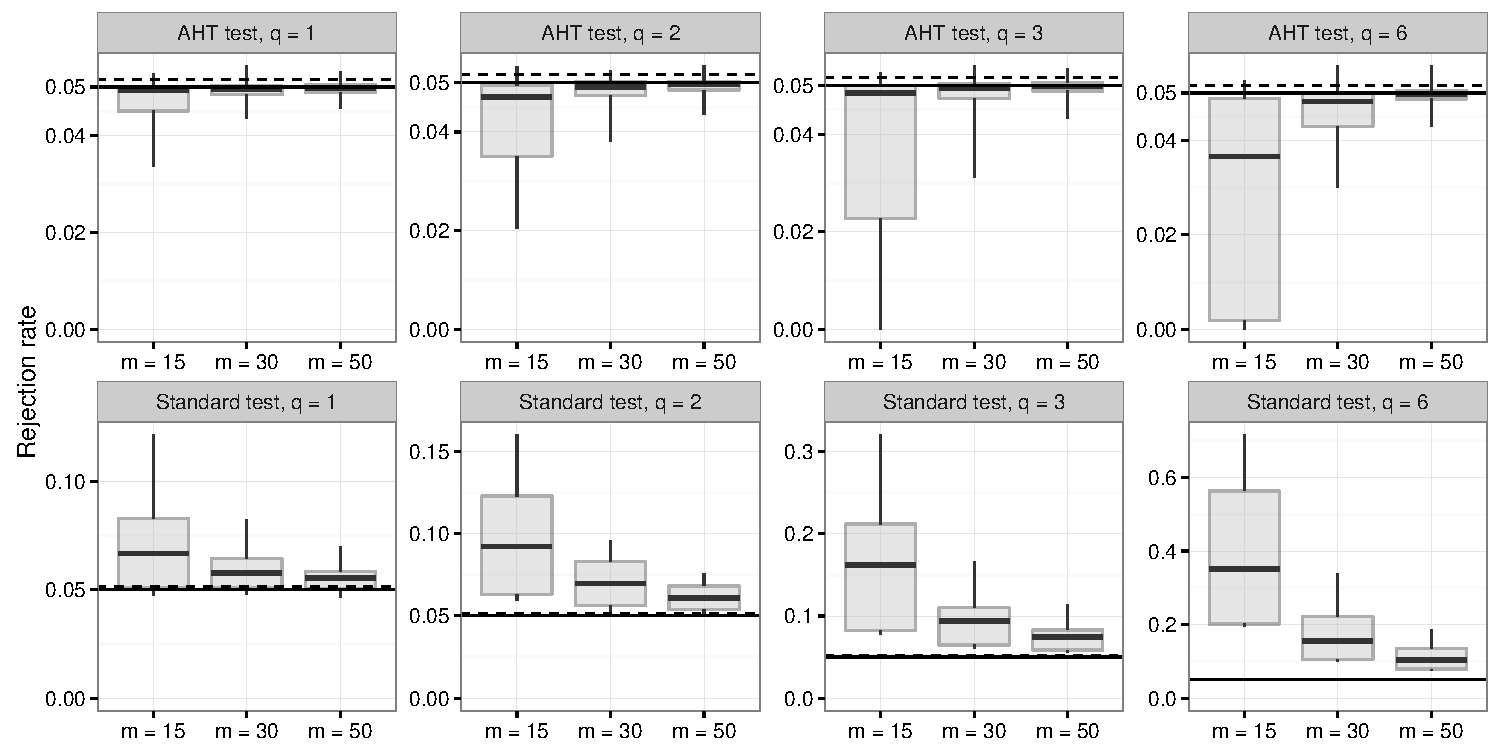
\includegraphics[width=\linewidth]{CR_fig/overview-1} 

}

\caption[Rejection rates of Standard and AHT tests, by dimension of hypothesis (]{Rejection rates of Standard and AHT tests, by dimension of hypothesis ($q$) and nominal type I error ($\alpha$).}\label{fig:overview}
\end{sidewaysfigure}


\end{knitrout}

The first finding is that the AHT test has Type I error close to the stated $\alpha$ level for all parameter combinations studied, whereas the standard test (based on the CR1 variance estimator and $m - 1$ degrees of freedom) does not. 
Figure \ref{fig:overview} illustrates this pattern, for constraints of varying dimension (from $q = 1$, in the first column, to $q = 6$, in the final column) and nominal $\alpha$ level (from .01, in the first row, to .10, in the last row). 
In each of these figures, the number of clusters varies from 15 to 50 (on the horizontal axis), the solid horizontal line indicates the stated $\alpha$ level and the dashed line indicates an upper confidence bound on simulation error.
It can be seen that the AHT test has Type I error near the stated $\alpha$ level, even with a small number of clusters.
When the number of clusters is very small, the Type I error can be smaller than the stated $\alpha$ level. 
Although there exist situations in which the error is above the simulation bound, the departures are typically small. For example, when $m = 15$ the rejection rates do not exceed 0.021 for $\alpha = .01$, 0.073 for $\alpha = .05$, and 0.134 for $\alpha = .10$.
The rejection rates are even closer to nominal for lower-dimensional constraints.
In comparison, the Type I error for the standard test can be markedly higher than the stated $\alpha$ level, particularly when the number of clusters is small or the dimension of the hypothesis is large. 
For example, for nominal $\alpha = .05$, the maximum Type I error ranges from 0.124 ($q = 1$) to 0.686 ($q = 6$) for data sets with 15 clusters.
Perhaps even more important for practice, even when there are 50 clusters, the rejection rate of the standard test can be far above the stated $\alpha$ level.
Again, focusing on the $\alpha = 0.05$ case, the maximum error ranges from 0.072 ($q = 1$) to 0.183 ($q = 6$).\todo{Beth, do you think reviewers are going to want to see the performance of CR3 here too?}

\begin{knitrout}
\definecolor{shadecolor}{rgb}{0.969, 0.969, 0.969}\color{fgcolor}\begin{sidewaysfigure}

{\centering 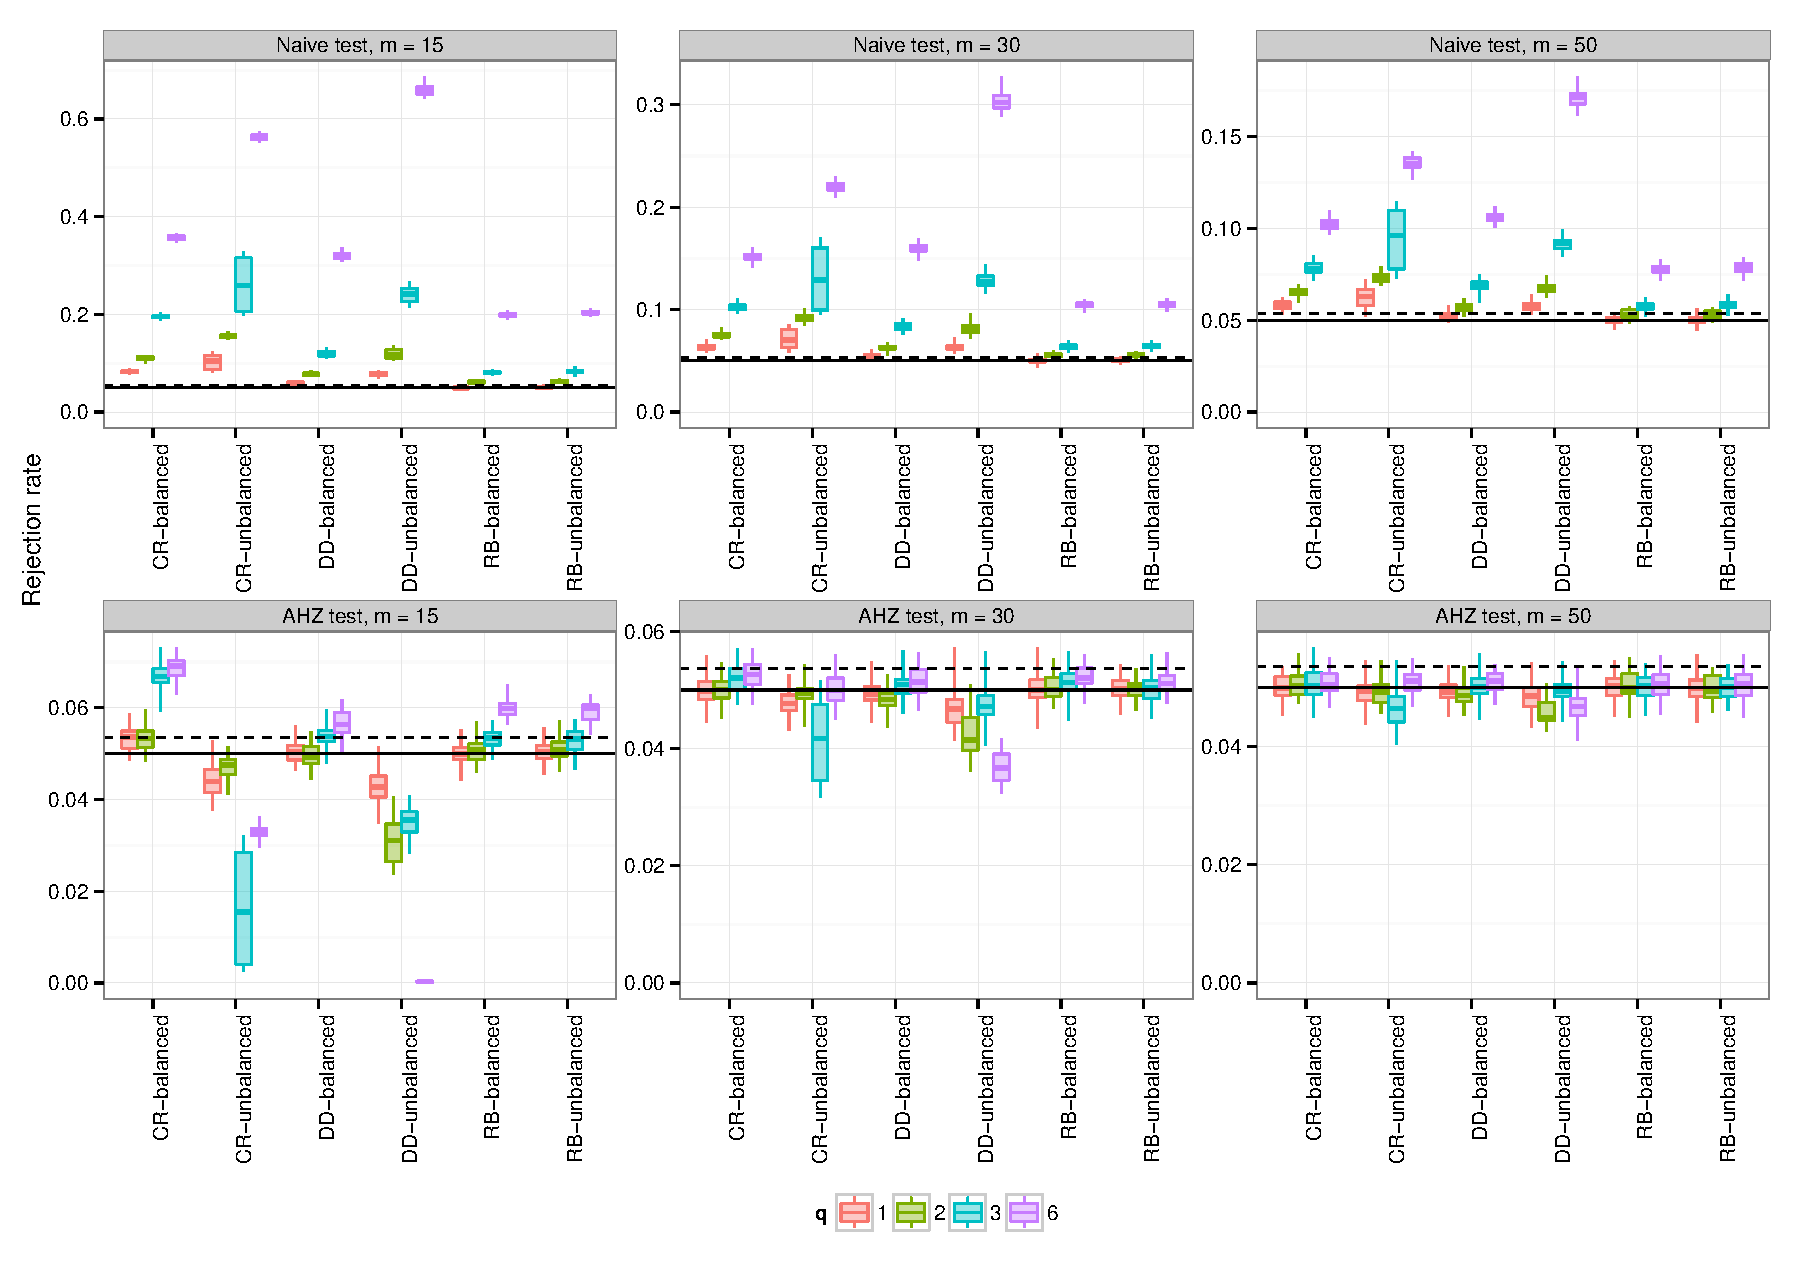
\includegraphics[width=\linewidth]{CR_fig/balance-1} 

}

\caption[Rejection rates of Standard and AHT tests, by study design and dimension of hypothesis (]{Rejection rates of Standard and AHT tests, by study design and dimension of hypothesis ($q$). CR = cluster-randomized design; DD = difference-in-differences design; RB = randomized block design; B = balanced; U = unbalanced.}\label{fig:balance}
\end{sidewaysfigure}


\end{knitrout}

In order to better understand the effects of different parameter combinations on the performance of both tests, Figure \ref{fig:balance} focuses on the $\alpha = 0.05$ case and breaks out the results by study design. The top row of the figure depicts the standard test, while the bottom row depicts the AHT test; columns correspond to the number of clusters.
Within each graph, results are given by study design (on the horizontal axis), with colors corresponding to the dimension of the test.
In the top panel, it can be seen that the rejection rate of the standard test increases with the dimension of the test ($q$) and the degree of unbalance in the study design.
Differences between the balanced and unbalanced designs are largest for the CR and DD designs, with smaller discrepancies in RB designs.
The bottom row of Figure \ref{fig:balance} displays results for the AHT test; here we focus on three trends.
First, the rejection rate of the AHT test usually increases as the dimension of the test increases, though never above 0.073.
Second, unbalanced designs led to rejection rates that were usually below the nominal $\alpha$---just the opposite of how the standard test is affected by unbalance. 
This trend is the strongest for CR and DD designs, where Type I error can be close to 0 at its minimum. 
Third, for studies with at least 30 clusters, rejection rates are very closes to nominal (between 0.032 and 0.057) across all conditions studied.

\begin{knitrout}
\definecolor{shadecolor}{rgb}{0.969, 0.969, 0.969}\color{fgcolor}\begin{sidewaysfigure}

{\centering 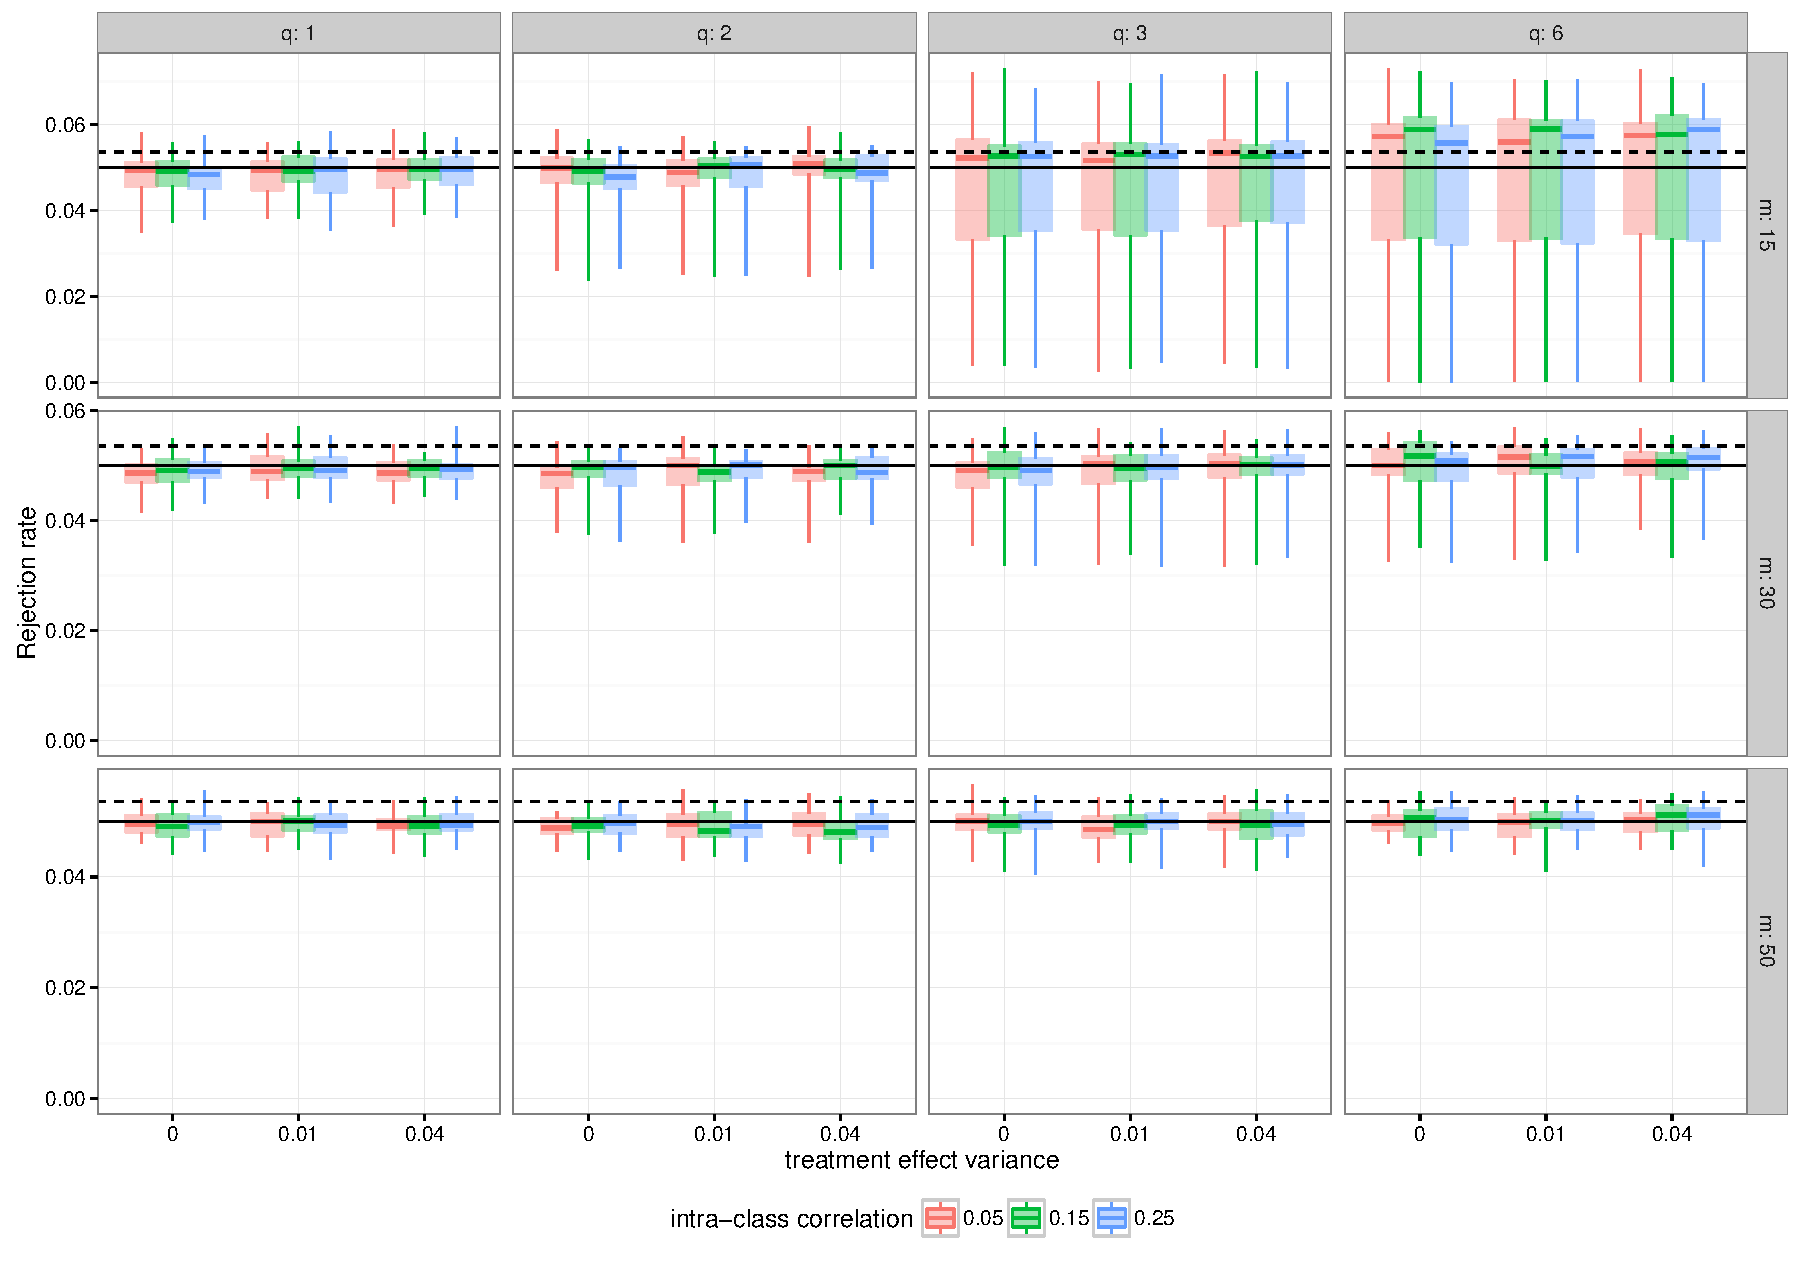
\includegraphics[width=\linewidth]{CR_fig/misspecification-1} 

}

\caption[Rejection rates of AHT test, by treatment effect variance and intra-class correlation]{Rejection rates of AHT test, by treatment effect variance and intra-class correlation.}\label{fig:misspecification}
\end{sidewaysfigure}


\end{knitrout}

Next, by simulating the errors across a variety of parameter combinations, we were also able to test the impact of misspecification of the working model on Type I error.
Because the CR2 correction and AHT degrees of freedom are both based on a working model with independent, homoskedastic errors, model misspecification increases with the true level of treatment effect variance ($\sigma_\delta^2$) and intra-class correlation ($\tau^2$).
Figure \ref{fig:misspecification} depicts Type I error rates for $\alpha = 0.05$ for the AHT test, with separate graphs according to the dimension $q$ of the test (columns) and the number of clusters (rows).
Within each panel, results are separated by the 9 combinations of $\sigma_\delta^2$ and $\tau^2$. 
It can be seen that the range of rejection rates remains very similar across the 9 error structures, with no clear pattern to the small differences that emerge.
These results follow closely those from Tipton and Pustejovsky (2015), which also found that even with extreme model misspecification the Type I error of the CR2S test was close to nominal. 

\begin{knitrout}
\definecolor{shadecolor}{rgb}{0.969, 0.969, 0.969}\color{fgcolor}\begin{figure}

{\centering 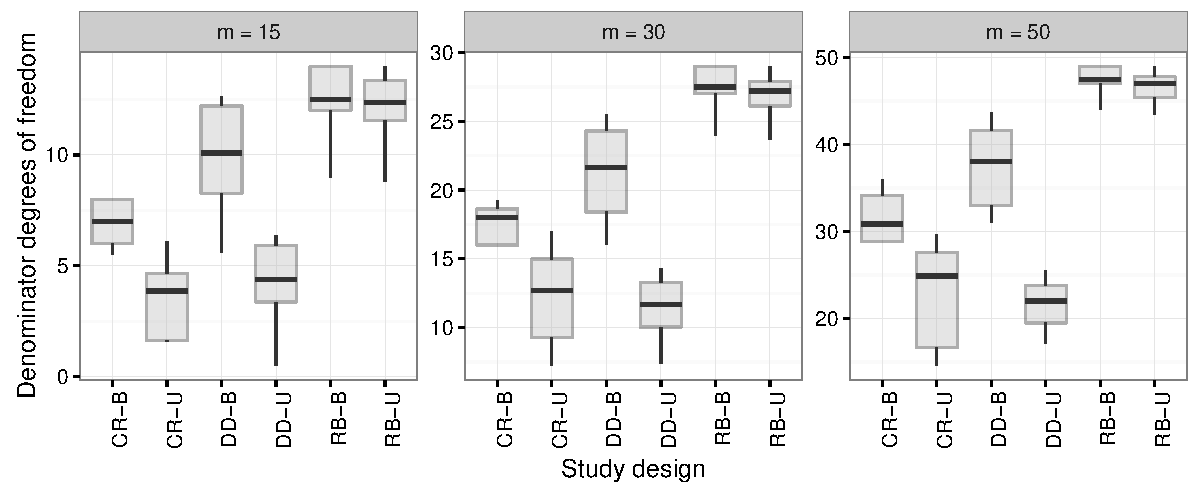
\includegraphics[width=\linewidth]{CR_fig/df-1} 

}

\caption[Range of denominator degrees of freedom for AHT test, by number of clusters and study design]{Range of denominator degrees of freedom for AHT test, by number of clusters and study design. CR = cluster-randomized design; DD = difference-in-differences design; RB = randomized block design; B = balanced; U = unbalanced.}\label{fig:df}
\end{figure}


\end{knitrout}

Finally, Figure \ref{fig:df} depicts the range of estimated degrees of freedom for the AHT test as a function of the simulated study design and number of clusters ($m$). 
Within each box plot, the degrees of freedom vary depending on the hypothesis tested, with constraints of larger dimension having lower degrees of freedom. 
It can be seen that the AHT degrees of freedom are often far less than $m - 1$ and that they are strongly affected by the pattern of treatment assignment and the degree of balance. The balanced and unbalanced RB designs generally had AHT degrees of freedom closest to $m - 1$ because the treatment effects being tested are all identified within each cluster. 
The balanced DD design usually had the next largest degrees of freedom because it involved contrasts between two patterns of treatment configuration, followed by the balanced CR design, which involved contrasts between three patterns of treatment configurations. 
For both of these designs, unbalance led to sharply reduced degrees of freedom.

These new simulation results have demonstrated that the standard robust Wald test, using the CR1 correction and $m - 1$ degrees of freedom, produces a wide range of rejection rates, often far in excess of the nominal Type I error. 
In contrast, the rejection rates of the AHT test are below or at most slightly above nominal, across the conditions that we have examined.
This is because the AHT test incorporates information about the covariate features into its estimated degrees of freedom, whereas the standard test does not.
An important question that remains then is how much the AHT and standard tests diverge in actual application.
In the next section, we compare the two tests in several examples, drawn from a range of recent empirical research.

\section{EXAMPLES}
\label{sec:examples}

This section presents three short examples that illustrate the performance of CRVE across a variety of applied contexts. 
In the first example, the effects of substantive interest involve between-cluster contrasts. 
The second example involves a cluster-robust Hausman test for differences between within- and across-cluster information. 
In the final example, the effects are identified within each cluster. 
In each example, we demonstrate the proposed AHT test for single- and multiple-parameter hypotheses and compare the results to the standard test based on the CR1 variance estimator and $m - 1$ degrees of freedom. 
The focus here is on providing insight into the conditions under which the AHT and standard estimators diverge in terms of three quantities of interest: the standard error estimates, the degrees of freedom estimates, and the stated p-values. 
Data files and replication code (in R) are available for each analysis as an online supplement.

\subsection{Achievement Awards demonstration} 

\citet{Angrist2009effects} reported results from a randomized trial in Israel that aimed to increase completion rates of the Bagrut, the national matriculation certificate for post-secondary education, among low-achieving high school students. 
In the Achievement Awards demonstration, 40 non-vocational high schools with low rates of Bagrut completion were selected from across Israel, including 10 Arab and 10 Jewish religious schools and 20 Jewish secular schools. 
The schools were then pair-matched based on 1999 rates of Bagrut completion, and within each pair one school was randomized to receive a cash-transfer program. 
In these treatment schools, seniors who completed certification were eligible for payments of approximately \$1,500. 
Student-level covariate and outcome data were drawn from administrative records for the school years ending in June of 2000, 2001, and 2002. 
The incentive program was in effect for the group of seniors in treatment schools taking the Bagrut exams in Spring of 2001, but the program was discontinued for the following year. 
We therefore treat completion rates for 2000 and 2002 as being unaffected by treatment assignment.
The primary outcome of interest is Bagrut completion. 

This study provides an opportunity to examine the AHT test in a situation in which the treatment was assigned at the cluster level, with a smaller number of clusters.
For simplicity, we restrict our analysis to the sample of female students, which reduces the total sample to 35 schools.
Following the original analysis of \citet{Angrist2009effects}, we allow the program's effects to vary depending on whether a students was in the upper or lower half of the distribution of prior-year academic performance. 
Letting $h = 1,2,3$ index the sector of each school (Arab religious, Jewish religious, or Jewish secular), we consider the following analytic model: 
\begin{equation}
\label{eq:AL_ATE}
y_{hitj} = z_{hit}\bm{r}_{hitj}'\bs\beta_h + \bm{s}_{hitj}'\bs\gamma + \gamma_{ht} + \mu_{hi} + \epsilon_{hitj}
\end{equation}
In this model for student $j$ in year $t$ in school $i$ in sector $h$, $z_{hit}$ is an indicator equal to one in the treatment schools for the 2001 school year and otherwise equal to zero; $\bm{r}_{hitj}$ is a vector of indicators for whether the student is in the lower or upper half of the distribution of prior academic performance; and $\bs\beta_h = \left(\beta_{1h}, \beta_{2h}\right)$ is a vector of average treatment effects for schools in sector $h$. 
The vector $\bm{s}_{hitj}$ includes the following individual student demographic measures: mother's and father's education, immigration status, number of siblings, and indicators for each quartile in the distribution of prior-year academic performance. 
The model also includes fixed effects $\gamma_{ht}$ for each sector in each year and $\mu_{hi}$ for each school. 

Based on Model (\ref{eq:AL_ATE}), we test four hypotheses, again with the goal of exploring the use of the AHT tests under a range of conditions. 
First, we assume that the program effects are constant across sector (i.e., $\bs\beta_1 = \bs\beta_2 = \bs\beta_3 = \bs\beta$) and test for whether the program affected completion rates for students in the upper half of the prior achievement distribution ($H_0: \beta_2 = 0$, with $q = 1$).
Second, we test for whether the program was effective in either half of the prior academic performance ($H_0: \bs\beta = 0$, with $q = 2$), still assuming that program effects are constant across sector. 
Third, we test for whether program effects in the upper half of the prior achievement distribution are moderated by school sector ($H_0: \beta_{21} = \beta_{22} = \beta_{23}$, with $q = 3$). 
Finally, we conduct a joint test for whether program effects in either half of the prior achievement distribution are moderated by school sector ($H_0: \bs\beta_1 = \bs\beta_2 = \bs\beta_3$, with $q = 4$). 



% latex table generated in R 3.2.3 by xtable 1.8-0 package
% Tue Jan 05 14:17:18 2016
\begin{table}[bth]
\centering
\begin{tabular}{lcrrr}
  \toprule
Hypothesis & Test & F & df & p \\ 
  \midrule
ATE - upper half (q = 1) & Standard & 5.746 & 34.00 & 0.02217 \\ 
   & AHT & 5.169 & 15.86 & 0.03726 \\ 
  ATE - joint (q = 2) & Standard & 3.848 & 34.00 & 0.03116 \\ 
   & AHT & 3.371 & 15.46 & 0.06096 \\ 
   \midrule
Moderation - upper half (q = 2) & Standard & 3.186 & 34.00 & 0.05393 \\ 
   & AHT & 0.091 & 3.19 & 0.91520 \\ 
  Moderation - joint (q = 4) & Standard & 8.213 & 34.00 & 0.00010 \\ 
   & AHT & 2.895 & 3.21 & 0.19446 \\ 
   \bottomrule
\end{tabular}
\caption{Tests of treatment effects in the Achievement Awards Demonstration} 
\label{tab:AAD}
\end{table}


Table \ref{tab:AAD} reports the results of all four hypothesis tests. 
These results indicate three important trends.
First, in the case of the first two hypotheses, the AHT test statistics are only slightly smaller than their standard counterparts, but the degrees of freedom are considerably smaller. 
These differences in degrees of freedom arise because the treatment was assigned at the cluster level, while the subgroups varied within each cluster. 
Second, the third and fourth hypotheses tests, which compared treatment effects across sectors and subgroups, are cases in which the AHT and standard tests diverge markedly.
For these cases, the AHT test statistic and degrees of freedom are both considerably smaller than those from the standard test. 
This reflects the degree of unbalance in allocations across sectors (19 Jewish secular, 7 Jewish religious, and 9 Arab religious schools), combined with cluster-level randomization. 
In combination, these smaller test statistics and degrees of freedom result in larger p-values for the AHT test when compared to the standard test.

\subsection{Effects of minimum legal drinking age on mortality} 

Our second example focues on panel data, using an example described in \citet{Angrist2014mastering}.
Using data from the Fatal Accident Reporting System maintained by the National Highway Traffic Safety Administration, we estimated the effects of changes in the minimum legal drinking age over the time period of 1970-1983 on state-level death rates resulting from motor vehicle crashes.\todo{Note about measure of legal drinking age.}
A standard difference-in-differences specification for such a state-by-year panel is
\begin{equation}
\label{eq:MLDA}
y_{it} = \bm{r}_{it}'\bs\beta + \gamma_t + \mu_i + \epsilon_{it}.
\end{equation}
In this model, time-point $t$ is nested within state $i$; the outcome $y_{it}$ is the number of deaths in motor vehicle crashes (per 100,000 residents) in state $i$ at time $t$; $\bm{r}_{it}$ is a vector of covariates; $\gamma_t$ is a fixed effect for time point $t$; and $\mu_i$ is an effect for state $i$. The vector $\bm{r}_{it}$ consists of a measure of the proportion of the population between the ages of 18 and 20 years who can legally drink alcohol and a measure of the beer taxation rate, both of which vary across states and across time.. 

We apply both random effects (RE) and fixed effects (FE) approaches to estimate the effect of lowering the legal drinking age. 
For the RE estimates, we use WLS with weights derived under the assumption that  $\mu_1,...,\mu_m$ are mutually independent, normally distributed, and independent of $\epsilon_{it}$ and $\bm{r}_{it}$.
We also report an artificial Hausman test \citep{Arellano1993on, Wooldridge2002econometric} for correlation between the covariates $\bm{r}_{it}$ and the state effects $\mu_i$. Such correlation creates bias in the RE estimator of the policy effect, thus necessitating the use of the FE estimator.
The artificial Hausman test amends model (\ref{eq:MLDA}) to include within-cluster deviations for the variables of interest, so that the estimating equation is
\begin{equation}
y_{it} = \bm{r}_{it}\beta + \bm{\ddot{r}}_{it}\bs\delta + \gamma_t + \mu_i + \epsilon_{it},
\end{equation}
where $\bm{\ddot{r}}_{it}$ denotes the within-cluster deviations of the covariate.
The parameter $\bs\delta$ captures the difference between the between-cluster and within-cluster estimates of $\bs\beta$. 
With this setup, the artificial Hausman test amounts to testing the null hypothesis that $\bs\delta = \bm{0}$, where $\bs\delta$ is estimated using RE.  



% latex table generated in R 3.2.3 by xtable 1.8-0 package
% Tue Jan 05 14:17:18 2016
\begin{table}[bth]
\centering
\begin{tabular}{lcrrr}
  \toprule
Hypothesis & Test & F & df & p \\ 
  \midrule
Random effects & Standard & 8.261 & 49.00 & 0.00598 \\ 
   & AHT & 7.785 & 24.74 & 0.00999 \\ 
  Fixed effects & Standard & 9.660 & 49.00 & 0.00313 \\ 
   & AHT & 9.116 & 22.72 & 0.00616 \\ 
   \midrule
Hausman test & Standard & 2.930 & 49.00 & 0.06283 \\ 
   & AHT & 2.489 & 8.69 & 0.13980 \\ 
   \bottomrule
\end{tabular}
\caption{Tests of effects of minimum legal drink age and Hausman specification test} 
\label{tab:MLDA}
\end{table}


Table \ref{tab:MLDA} displays the results of the tests for the policy variable and the Hausman tests for each model specification. 
The results of the policy effect tests are quite similar across specifications and versions of the test. 
Of note is that, for both the RE and FE estimates, the AHT tests have only half the degrees of freedom of the corresponding standard tests. 
For the artificial Hausman test, the AHT test has fewer than 9 degrees of freedom, which leads to a much larger p-value compared to using the standard test based on CR1. 

\subsection{Tennessee STAR class-size experiment.} 

The final example demonstrates an application in which the AHT and standard tests lead to similar results. The Tennessee STAR class size experiment is one of the most intensively studied interventions in education \citep[for a detailed review, see][]{Schanzenbach2006what}.  The experiment involved students in kindergarten through third grade across 79 schools. Within each school, students and their teachers were randomized equally to one of three conditions: small class-size (targeted to have 13-17 students), regular class-size, or regular class-size with an aide.
Subsequent research has focused on the effects of these conditions on kindergarten reading, math, and word recognition \citep{Achilles2008tennessee}; high school test scores \citep{Schanzenbach2006what}; college entrance exam participation \citep{Krueger2001effect}; and home ownership and earnings \citep{Chetty2011how}, among other outcomes.

The STAR experiment involved three treatment conditions and multiple outcomes, providing a scenario where both t-tests (with $q = 1$) and F-tests with varying constraint dimensions can be applied. 
For simplicity, we focus only on the subgroup of students who were in kindergarten during the first year of the study, and on three outcomes measured at the end of the kindergarten year: reading, word recognition, and math \citep{Achilles2008tennessee}. 
Outcome scores are standardized to percentile ranks, following \citet{Krueger2001effect}.
The analytic model is: 
\begin{equation}
y_{ijk} = \bm{r}_{ij}'\bs\beta_k + \bm{s}_{ij}'\bs\gamma_0 + \gamma_k + \mu_i + \epsilon_{ijk}, 
\end{equation}
where $y_{ijk}$ is the percentile rank on outcome $k$ for student $j$ in school $i$; $\bm{r}_{ij}$ includes indicators for the small-class and regular-plus-aide conditions; $\bm{s}_{ij}$ includes student demographic covariates (i.e., free or reduced-price lunch status; race; gender; age); $\gamma_k$ is a fixed effect for outcome $k$; and $\mu_i$ is a fixed effect for school $i$. 
In this model, $\beta_{1k}$ represents the average effect of being in a small class and $\beta_{2k}$ represents the average of effect of being in a regular class with an aid, in each case compared to a regular-size class without an aid.

Using this model, we test four distinct hypotheses that vary in dimension from $q = 1$ to $q = 6$. 
First, using only the math achievement scores, we test the effects of small class size ($H_0: \beta_{11} = 0$) while maintaining the assumption that the additional classroom aide has no effect on student achievement (i.e., constraining $\beta_{21} = 0$). 
Second, again only using the data for outcome $k$, we test the hypothesis that there are no differences across the three class-size conditions (i.e., $H_0: \bs\beta_1 = \bm{0}$). 
Third, combining the data across all three outcomes, we test the hypothesis that small class size (vs regular and regular plus aide) had no effects on any outcome (i.e., $\beta_{11} = \beta_{12} = \beta_{13} = 0$).
Finally, we test the hypothesis that there are no differences across the three class-size conditions on any outcome (i.e., $H_0: \bs\beta_1 = \bs\beta_2 = \bs\beta_3 = \bm{0}$). 
The third and fourth tests use the seemingly unrelated regression (SUR) framework, in which separate treatment effects are estimated for each outcome, but the student demographic effects and school fixed effects are pooled across outcomes. 
In all models, we estimated $\bs\beta_k$ and $\bs\gamma$ after absorbing the school fixed effects and clustering the standard errors by school.



% latex table generated in R 3.2.3 by xtable 1.8-0 package
% Tue Jan 05 14:17:18 2016
\begin{table}[tbh]
\centering
\begin{tabular}{lllrrr}
  \toprule
Outcome & Effect & Test & F & df & p \\ 
  \midrule
Math & Small class (q=1) & Standard & 13.624 & 78.0 & 0.00041 \\ 
   &  & AHT & 13.590 & 69.0 & 0.00045 \\ 
   & Small class and classroom aide (q=2) & Standard & 6.838 & 78.0 & 0.00183 \\ 
   &  & AHT & 6.725 & 68.6 & 0.00215 \\ 
   \midrule
Combined & Small class (q=3) & Standard & 6.408 & 78.0 & 0.00062 \\ 
   &  & AHT & 6.206 & 67.0 & 0.00088 \\ 
   & Small class and classroom aide (q=6) & Standard & 3.284 & 78.0 & 0.00622 \\ 
   &  & AHT & 3.042 & 64.9 & 0.01103 \\ 
   \bottomrule
\end{tabular}
\caption{Tests of treatment effects in the Tennessee STAR class size experiment} 
\label{tab:STAR}
\end{table}


Table \ref{tab:STAR} displays the results for a representative subset of these hypothesis tests, using either the standard test (with CR1) or the AHT test (with CR2).
These results illustrate two important points regarding the use of the AHT test in practice.
First, across all three analyses, the AHT t- and F-tests are only typically slightly smaller than the corresponding standard test.
%This trend is common because the CR2 adjustments to the variance estimator are typically small in scope.\todo{This needs to be qualified--Angrist \& Lavy found that the CR2 standard errors were considerably larger than the unadjusted SEs!}
Second, if treatment is randomly allocated in approximately equal proportions within each cluster---as occurred in the TN STAR experiment---the degrees of freedom for the AHT tests are only slightly smaller than those for the standard tests.
In combination with the rather large sample size of 79 schools, these differences have only a minimal effect on the p-values for these tests. 
As the previous two examples illustrate, however, the similarity between these tests is not common, and is a result only of the design of the study, indicating that the standard test is best used only in experiments randomized within clusters. 

\section{Conclusion}
\label{sec:conclusion}

Across the field of economics, empirical studies often involve modeling data with a correlated error structure. 
Correlated errors arise in the analysis of multi-stage samples, cluster-randomized trials, panel data, and regression discontinuities with discrete forcing variables, among other study designs. 
It is now routine to handle dependent error structures by using cluster-robust variance estimation, which provides asymptotically valid standard errors and hypothesis tests without making strong parametric assumptions about the error structure. 
However, a growing body of recent work has drawn attention to the shortcomings of CRVE methods when the data include only a small or moderate number of independent clusters \citep{Cameron2008bootstrap, Cameron2015practitioners, Imbens2015robust, Webb2013wild}. 
In particular, Wald tests based on CRVE can have rejection rates far in excess of the nominal Type I error. 
This problem is compounded by the fact that the performance of standard Wald tests depends on features of the study design beyond just the total number of clusters, which can make it difficult to determine whether standard, asymptotic valid CRVE methods are accurate. 


One promising solution to this problem is to use the bias-reduced linearization variance estimator (i.e., CR2) proposed by \citet{Bell2002bias}, which corrects the CRVE so that it is exactly unbiased under an analyst-specified working model for the error structure, together with degrees of freedom estimated based on the same working model.
In this paper, we have demonstrated that the CR2 variance estimator is a fully general solution, which can be applied even in models with fixed effects in multiple dimensions. 
Our re-formulation of the bias-reduced linearization criteria also makes clear how to calculate the CR2 correction when the model includes fixed effects, whether those fixed effects are estimated by OLS or are instead absorbed before estimating the target regression parameters.  
Finally, we have proposed a method for testing hypotheses that involve multiple constraints on regression parameters, based on an approximation that generalizes the existing Satterthwaite approximation for t-tests.  
With the modifications and extensions proposed in this paper, the CR2 variance estimator and small-sample testing procedures can be applied in a wide range of analytic models---essentially, any model estimated by ordinary or weighted least squares. 

We join \citet{Imbens2015robust} in arguing that the CR2 estimator and corresponding estimated degrees of freedom for hypothesis tests should be applied routinely, whenever analysts use CRVE and hypothesis tests based thereon. 
Because the performance of standard CRVE methods depends on features of the study design, the total number of clusters in the data is an insufficient guide to whether small-sample corrections are needed. 
Instead, the clearest way to determine whether small-sample corrections are needed is simply to calculate them.
The proposed AHT test involves two adjustments: use of the CR2 adjustment for the variance estimator and use of estimated degrees of freedom. 
Our simulation study illustrates that the combined result of these adjustments results in an AHT test with Type I error close to the stated $\bs\alpha$ level. 
Furthermore, our empirical examples illustrate that the degrees of freedom adjustment has a relatively larger influence on small-sample performance.
These degrees of freedom can be much smaller than the number of clusters, particularly when the covariates involved in the test involve high leverage or are unbalanced across clusters.
The estimated degrees of freedom are indicative of the precision of the standard errors, and thus provide diagnostic information that is similar to the effective sample size measure proposed by \citet{Carter2013asymptotic}. 
We therefore recommend that the degrees of freedom be reported along with standard errors and $p$-values whenever the method is applied.

The idea of developing small-sample adjustments based on a working model may seem strange to analysts accustomed to using CRVE---after all, the whole point of clustering standard errors is to avoid making assumptions about the error structure.
However, simulation studies reported here and elsewhere \citep{Tipton2015small-t, Tipton2015small-F} have demonstrated that the approach is actually robust to a high degree of misspecification in the working model. 
Furthermore, while the working model provides necessary ``scaffolding'' when the number of clusters is small, its  influence tends to fall away as the number of clusters increases, so that the CR2 estimator and AHT maintain the same asymptotic robustness as standard CRVE methods. 

One outstanding problem with the CR2 variance estimator is that it can become computationally costly (or even infeasible) when the within-cluster sample sizes are large \citep{Mackinnon2014wild}. 
For example, \citet{Bertrand2004how} analyzed micro-level data from a 21-year panel of current population survey data, with clustering by state. Their data included some state-level clusters with over $n_i = 10,000$ individual observations. 
The CR2 adjustment matrices have dimension $n_i \times n_i$, and would be very expensive to compute in this application. 
Methods for improving the computational efficiency of the CR2 variance estimator (or alternative estimators that have similar performance to CR2), should be investigated further. 

This paper has developed the CR2 estimator and AHT testing procedure for weighted least squares estimation of linear regression models. 
Extensions to linear regression models with clustering in multiple, non-nested dimensions \citep[cf.][]{Cameron2011robust} appear to be possible, and their utility should be further investigated. 
\citet{McCaffrey2006improved} have proposed extensions to bias-reduced linearization for use with generalized estimating equations, and future work should consider further extensions to other classes of estimators, including two-stage least squares and generalized method of moments. 
\citet{McCaffrey2006improved} also found that for single-parameter hypotheses, a saddlepoint approximation to the Wald test statistic provides even more accurate rejection rates than the Satterthwaite approximation given in Equation (\ref{eq:nu_model}). 
It would be interesting to investigate whether the saddlepoint approximation could be extended to handle multiple-parameter constraints, although this appears to be far from straight-forward. 

\todo[inline]{Should we talk about Wild bootstrap at all here?}


\appendix

\section{BRL adjustment matrices}
\label{app:theorems}

This appendix provides proof of the two theorems from Section \ref{sec:BRL}. 

\subsection{Proof of Theorem \ref{thm:BRL_FE}}

The Moore-Penrose inverse of $\bm{B}_i$ can be computed from its eigen-decomposition. Let $b \leq n_i$ denote the rank of $\bm{B}_i$. 
Let $\bs\Lambda$ be the $b \times b$ diagonal matrix of the positive eigenvalues of $\bm{B}_i$ and $\bm{V}$ be the $n_i \times b$ matrix of corresponding eigen-vectors, so that $\bm{B}_i = \bm{V}\bs\Lambda\bm{V}'$. 
Then $\bm{B}_i^+ = \bm{V}\bs\Lambda^{-1}\bm{V}'$ and $\bm{B}_i^{+1/2} = \bm{V}\bs\Lambda^{-1/2}\bm{V}'$. Now, observe that 
\begin{align}
\label{eq:step1}
\bm{\ddot{R}}_i' \bm{W}_i \bm{A}_i \left(\bm{I} - \bm{H_X}\right)_i \bs\Phi \left(\bm{I} - \bm{H_X}\right)_i' \bm{A}_i' \bm{W}_i \bm{\ddot{R}}_i &= \bm{\ddot{R}}_i' \bm{W}_i \bm{D}_i \bm{B}_i^{+1/2} \bm{B}_i \bm{B}_i^{+1/2} \bm{D}_i' \bm{W}_i \bm{\ddot{R}}_i \nonumber \\
&= \bm{\ddot{R}}_i' \bm{W}_i \bm{D}_i \bm{V}\bm{V}' \bm{D}_i' \bm{W}_i \bm{\ddot{R}}_i. 
\end{align}

Because $\bm{D}_i$, and $\bs\Phi$ are positive definite and $\bm{B}_i$ is symmetric, the eigen-vectors $\bm{V}$ define an orthonormal basis for the column span of $\left(\bm{I} - \bm{H_{\ddot{X}}}\right)_i$.
We now show that $\bm{\ddot{U}}_i$ is in the column space of $\left(\bm{I} - \bm{H_X}\right)_i$. 
Let $\bm{Z}_i$ be an $n_i \times (r + s)$ matrix of zeros. 
Let $\bm{Z}_k = - \bm{\ddot{U}}_k \bm{L}^{-1}\bm{M}_{\bm{\ddot{U}}}^{-1}$, for $k \neq j$ and take $\bm{Z} = \left(\bm{Z}_1',...,\bm{Z}_m'\right)'$. 
Now observe that $\left(\bm{I} - \bm{H_T}\right) \bm{Z} = \bm{Z}$. 
It follows that 
\begin{align*}
\left(\bm{I} - \bm{H_X}\right)_i \bm{Z} &= \left(\bm{I} - \bm{H_{\ddot{U}}}\right)_i \left(\bm{I} - \bm{H_T}\right) \bm{Z} = \left(\bm{I} - \bm{H_{\ddot{U}}}\right)_i \bm{Z} \\
&= \bm{Z}_i - \bm{\ddot{U}}_i\bm{M_{\ddot{U}}}\sum_{k=1}^m \bm{\ddot{U}}_k'\bm{W}_k\bm{Z}_k = \bm{\ddot{U}}_i\bm{M_{\ddot{U}}} \left(\sum_{k \neq j} \bm{\ddot{U}}_k' \bm{W}_k \bm{\ddot{U}} \right) \bm{L}^{-1}\bm{M}_{\bm{\ddot{U}}}^{-1} \\
&= \bm{\ddot{U}}_i.
\end{align*}
Thus, there exists an $N \times (r + s)$ matrix $\bm{Z}$ such that $\left(\bm{I} - \bm{H_{\ddot{X}}}\right)_i \bm{Z} = \bm{\ddot{U}}_i$, i.e., $\bm{\ddot{U}}_i$ is in the column span of $\left(\bm{I} - \bm{H_X}\right)_i$. Because $\bm{D}_i \bm{W}_i$ is positive definite and $\bm{\ddot{R}}_i$ is a sub-matrix of $\bm{\ddot{U}}_i$, $\bm{D}_i\bm{W}_i\bm{\ddot{R}}_i$ is also in the column span of $\left(\bm{I} - \bm{H_X}\right)_i$. It follows that 
\begin{equation}
\label{eq:step2}
\bm{\ddot{R}}_i' \bm{W}_i \bm{D}_i \bm{V}\bm{V}' \bm{D}_i' \bm{W}_i \bm{\ddot{R}}_i = \bm{\ddot{R}}_i' \bm{W}_i \bs\Phi_i \bm{W}_i \bm{\ddot{R}}_i.
\end{equation}
Substituting (\ref{eq:step2}) into (\ref{eq:step1}) demonstrates that $\bm{A}_i$ satisfies criterion (\ref{eq:CR2_criterion}).

Under the working model, the residuals from cluster $i$ have mean $\bm{0}$ and variance \[
\Var\left(\bm{\ddot{e}}_i\right) = \left(\bm{I} - \bm{H_X}\right)_i \bs\Phi \left(\bm{I} - \bm{H_X}\right)_i',\] 
It follows that 
\begin{align*}
\E\left(\bm{V}^{CR2}\right) &= \bm{M_{\ddot{R}}}\left[\sum_{i=1}^m \bm{\ddot{R}}_i' \bm{W}_i \bm{A}_i \left(\bm{I} - \bm{H_X}\right)_i \bs\Phi \left(\bm{I} - \bm{H_X}\right)_i' \bm{A}_i \bm{W}_i \bm{\ddot{R}}_i \right] \bm{M_{\ddot{R}}} \\
&= \bm{M_{\ddot{R}}}\left[\sum_{i=1}^m \bm{\ddot{R}}_i' \bm{W}_i \bs\Phi_i \bm{W}_i \bm{\ddot{R}}_i \right] \bm{M_{\ddot{R}}} \\
&= \Var\left(\bs{\hat\beta}\right)
\end{align*}

\subsection{Proof of Theorem \ref{thm:absorb}}

From the fact that $\bm{\ddot{U}}_i'\bm{W}_i\bm{T}_i = \bm{0}$ for $i = 1,...,m$, it follows that \begin{align*}
\bm{B}_i &= \bm{D}_i \left(\bm{I} - \bm{H_{\ddot{U}}}\right)_i \left(\bm{I} - \bm{H_T}\right) \bs\Phi \left(\bm{I} - \bm{H_T}\right)' \left(\bm{I} - \bm{H_{\ddot{U}}}\right)_i' \bm{D}_i'\\
&= \bm{D}_i \left(\bm{I} - \bm{H_{\ddot{U}}} - \bm{H_T}\right)_i \bs\Phi \left(\bm{I} - \bm{H_{\ddot{U}}} - \bm{H_T}\right)_i' \bm{D}_i' \\
&= \bm{D}_i \left(\bs\Phi_i - \bm{\ddot{U}}_i \bm{M_{\ddot{U}}}\bm{\ddot{U}}_i' - \bm{T}_i \bm{M_T}\bm{T}_i'\right)\bm{D}_i'
\end{align*}
and 
\begin{equation}
\label{eq:B_i_inverse}
\bm{B}_i^+ = \left(\bm{D}_i'\right)^{-1} \left(\bs\Phi_i - \bm{\ddot{U}}_i \bm{M_{\ddot{U}}}\bm{\ddot{U}}_i' - \bm{T}_i \bm{M_T}\bm{T}_i'\right)^+ \bm{D}_i^{-1}.
\end{equation}
Let $\bs\Psi_i = \left(\bs\Phi_i - \bm{\ddot{U}}_i \bm{M_{\ddot{U}}}\bm{\ddot{U}}_i'\right)^+$.
Using a generalized Woodbury identity \citep{Henderson1981on}, \[
\bs\Psi_i = \bm{W}_i + \bm{W}_i \bm{\ddot{U}}_i \bm{M_{\ddot{U}}}\left(\bm{M_{\ddot{U}}} - \bm{M_{\ddot{U}}} \bm{\ddot{U}}_i' \bm{W}_i \bm{\ddot{U}}_i \bm{M_{\ddot{U}}}\right)^+ \bm{M_{\ddot{U}}}\bm{\ddot{U}}_i'\bm{W}_i. \]
It follows that $\bs\Psi_i \bm{T}_i = \bm{W}_i \bm{T}_i$. 
Another application of the generalized Woodbury identity gives 
\begin{align*}
\left(\bs\Phi_i - \bm{\ddot{U}}_i \bm{M_{\ddot{U}}}\bm{\ddot{U}}_i' - \bm{T}_i \bm{M_T}\bm{T}_i'\right)^+ &= \bs\Psi_i + \bs\Psi_i \bm{T}_i \bm{M_T}\left(\bm{M_T} - \bm{M_T}\bm{T}_i' \bs\Psi_i \bm{T}_i \bm{M_T}\right)^+ \bm{M_T} \bm{T}_i' \bs\Psi_i \\
&= \bs\Psi_i + \bm{W}_i \bm{T}_i \bm{M_T}\left(\bm{M_T} - \bm{M_T}\bm{T}_i' \bm{W}_i \bm{T}_i\bm{M_T}\right)^+ \bm{M_T} \bm{T}_i' \bm{W}_i \\
&= \bs\Psi_i.
\end{align*}
The last equality follows from the fact that $\bm{T}_i \bm{M_T}\left(\bm{M_T} - \bm{M_T}\bm{T}_i' \bm{W}_i \bm{T}_i\bm{M_T}\right)^{-} \bm{M_T} \bm{T}_i' = \bm{0}$ because the fixed effects are nested within clusters. 
Substituting into (\ref{eq:B_i_inverse}), we then have that $\bm{B}_i^+ = \left(\bm{D}_i'\right)^{-1} \bs\Psi_i \bm{D}_i^{-1}$. 
But \[
\bm{\tilde{B}}_i = \bm{D}_i \left(\bm{I} - \bm{H_{\ddot{U}}}\right)_i \bs\Phi \left(\bm{I} - \bm{H_{\ddot{U}}}\right)_i' \bm{D}_i' = \bm{D}_i \left(\bs\Phi_i - \bm{\ddot{U}}_i\bm{M_{\ddot{U}}} \bm{\ddot{U}}_i'\right) \bm{D}_i' = \bm{D}_i \bs\Psi_i^+ \bm{D}_i',
\]
and so $\bm{B}_i^+ = \bm{\tilde{B}}_i^+$. It follows that $\bm{A}_i = \bm{\tilde{A}}_i$ for $i = 1,...,m$. 

\section{Details of simulation study}
\label{app:simulations}

This appendix provides further details regarding the design of the simulations reported in Section \ref{sec:simulation}. The simulations examined six distinct study designs. Outcomes are measured for $n$ units (which may be individuals, as in a cluster-randomized or block-randomized design, or time-points, as in a difference-in-differences panel) in each of $m$ clusters under one of three treatment conditions. Suppose that there are $G$ groups of units that share an identical pattern of treatment assignments, each of size $m_g$. Let $n_{ghi}$ denote the number of units at which cluster $i$ in group $g$ is observed under condition $h$, for $i=1,...,m$, $g = 1,...,G$, and $h = 1,2,3$. The following six designs were simulated:
\begin{enumerate}
\item A balanced, block-randomized design, with an un-equal allocation within each block. In the balanced design, the treatment allocation is identical for each block, with $G = 1$, $m_1 = m$, $n_{11i} = n / 2$, $n_{12i} = n / 3$, and $n_{13i} = n / 6$.
\item An unbalanced, block-randomized design, with two different patterns of treatment allocation. Here, $G = 2$,  $m_1 = m_2 = m / 2$, $n_{11i} = n / 2$, $n_{12i} = n / 3$, $n_{13i} = n / 6$, $n_{21i} = n / 3$, $n_{22i} = 5 n / 9$, and $n_{23i} = n / 9$.
\item A balanced, cluster-randomized design, in which units are nested within clusters and an equal number of clusters are assigned to each treatment condition. Here, $G = 3$, $m_g = m / 3$, and $n_{ghi} = n$ for $g = h$ and zero otherwise.
\item An unbalanced, cluster-randomized design, in which units are nested within clusters but the number of clusters assigned to each condition is not equal. Here, $G = 3$; $m_1 = 0.5 m, m_2 = 0.3 m, m_3 = 0.2 m$; and $n_{ghi} = n$ for $g = h$ and zero otherwise. 
\item A balanced difference-in-differences design, with two patterns of treatment allocation ($G = 2$) and clusters allocated equally to each pattern ($m_1 = m_2 = m / 2$). Here, half of the clusters are observed under the first treatment condition only ($n_{11i} = n$) and the remaining half are observed under all three conditions, with $n_{21i} = n / 2$, $n_{22i} = n / 3$, and $n_{23i} = n / 6$.
\item An unbalanced difference-in-differences design, again with two patterns of treatment allocation ($G = 2$), but where $m_1 = 2 m / 3$ clusters are observed under the first treatment condition only ($n_{11i} = n$) and the remaining $m_2 = m / 3$ clusters are observed under all three conditions, with  $n_{21i} = n / 2$, $n_{22i} = n / 3$, and $n_{23i} = n / 6$.
\end{enumerate}

\bibliographystyle{agsm}
\bibliography{bibliography}

\end{document}

